% Activate the following line by filling in the right side. If for example the name of the root file is Main.tex, write
% "...root = Main.tex" if the chapter file is in the same directory, and "...root = ../Main.tex" if the chapter is in a subdirectory.
 
% !TEX root = ../thesis.tex 

\chapter{The origin and correction of partial volume effects}
\label{pvec_chapter}

\section{Introduction}
\subsection{Interpretations of the partial volume effect}

PVE are a consequence of the limited spatial resolution of physiological imaging data in relation to the length scale of structures of interest. Low spatial resolution arises either due to modality-specific mechanisms (a high PSF in the case of PET), or as a means of mitigating low SNR (in the case of ASL). 

There are multiple possible interpretations of how PVE affect the acquisition of physiological imaging data. One interpretation is that they introduce a dependence between the discretisation basis of the data and the distribution of acquired signal. This is because the signal in a voxel is linearly proportional to the tissue PV within that voxel, and the tissue PVs themselves depend on the voxel grid (according to the intersection made with the structure in question). This is illustrated in figure \ref{CBF_with_PVE_demo}, in which a representative GM CBF map with PVE is simulated by drawing CBF values from a normal distribution and multiplying by a set of ground truth PV estimates. The accompanying scatter plot shows a linear relationship between the PV fraction of a given voxel and its CBF value, a relationship that arises purely due to the discretisation basis of the data. The consequence of this is that any change to the subject anatomy / voxel grid intersection (for example, movement during an acquisition) will lead to a change in the PVs associated with said grid, thereby changing the distribution of PVE within the data. To continue the example given in figure \ref{CBF_with_PVE_demo}, this is equivalent to drawing a new set of samples, modulated by the new PVs, from the same underlying parameter distribution.

\begin{figure}
\centering
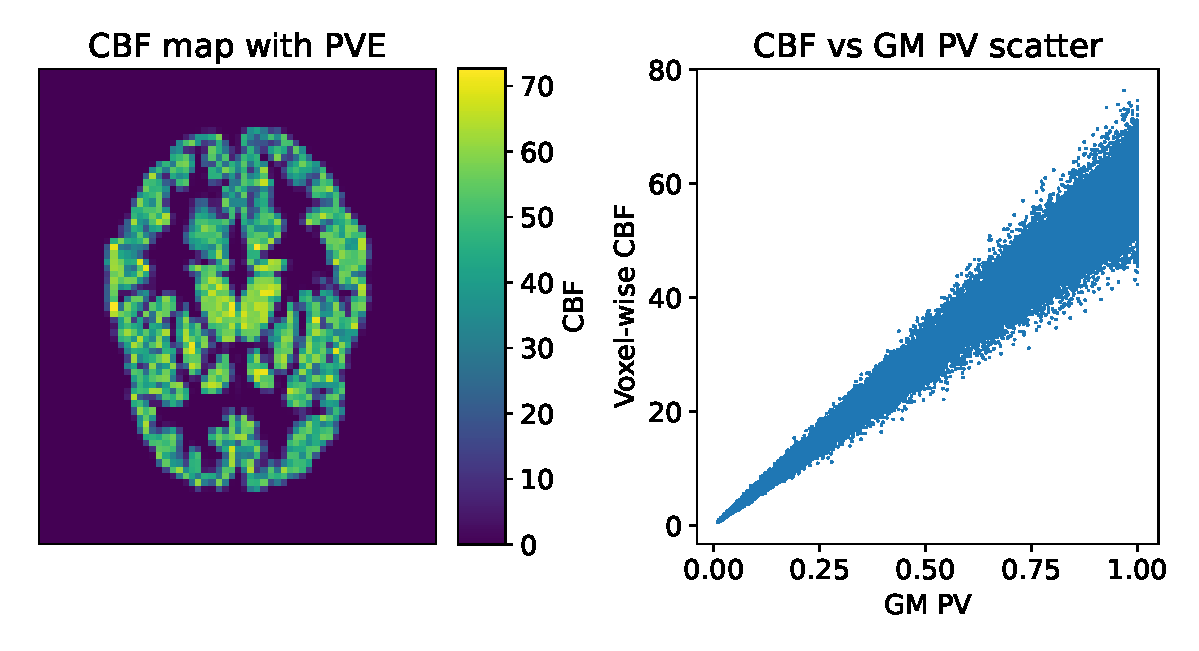
\includegraphics[width = 0.75\textwidth]{CBF_with_PVE.eps}
\caption{Left: GM CBF map with PVE, simulated by drawing CBF samples from a normal distribution with mean 60 and standard deviation 5. These samples are multiplied with a set of ground truth GM PV estimates to give a representative CBF map, as would be obtained from ASL data for example. Right: a scatter plot of voxel PV against CBF value. Even allowing for the variance within the CBF samples drawn from the distribution, a strong relationship between voxel PV and voxel CBF is observed.}
\label{CBF_with_PVE_demo}
\end{figure}

An alternative interpretation of PVE is that they increase the within-class variance of measurements obtained from a given tissue, as illustrated in figure \ref{CBF_PVE_hist_simple}. Once again the same ground truth distribution of GM CBF is assumed, from which CBF maps are simulated using ground truth PV maps at various resolutions (0.7mm, 2.1mm and 3.5mm isotropic). As voxel size increases, it can be seen that the histogram of voxel-wise CBF alters: there are fewer `pure' GM voxels, and hence fewer voxels with high CBF, which leads to greater within-class variance. In quantitative terms, the modal value of the distribution is reduced and variance increased. 

\begin{figure}
\centering
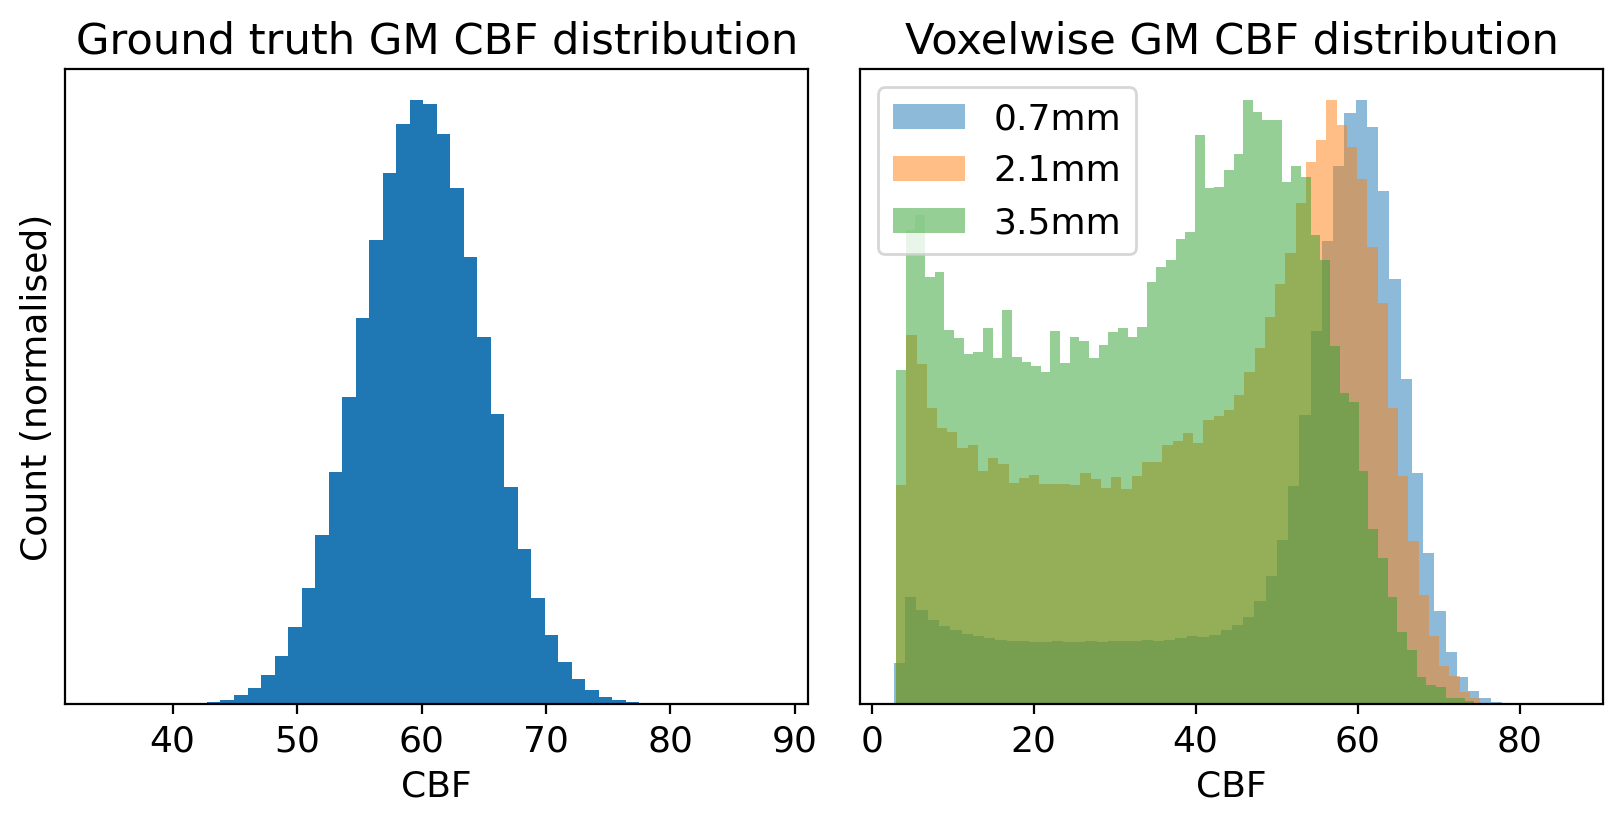
\includegraphics[width = 0.75\textwidth]{CBF_PVE_hists.png}
\caption{Left: a ground truth distribution of GM CBF, normal with mean 60 and standard deviation 5. Samples from this distribution are multiplied with a set of ground truth GM PV estimates at various resolutions to give a representative CBF map, as would be obtained via ASL imaging for example. Right: histograms of voxel-wise CBF at each resolution. As voxel size increases, the histograms become more spread out (within-class variance is increased) and the modal value decreases. The vertical axis has been normalised for clarity.}
\label{CBF_PVE_hist_simple}
\end{figure}

\subsection{The consequences of resampling}

Typical processing pipelines for physiological data make use of motion correction and registration. The former operation is required to combine data from multiple modalities or resolutions (for example, applying a structural ROI from an MRI image to PET data). The latter is desirable to reduce the effects of patient motion during lengthy acquisitions (themselves a means of improving SNR). Both of these operations require resampling, a mathematical operation that is used to transform data between voxel grids.  

Resampling is achieved via the use of high-dimensional interpolation between the coordinates of the voxel grids; in all of the following discussion linear interpolation in three dimensions is assumed (though it is possible to use other basis functions for interpolation, for example splines or sinc functions). Any transformation of a volumetric image may be interpreted as a transformation of the voxel grid upon which the data is currently represented. For example, to translate an image of the brain by 1mm along any axis within a voxel grid, one can hold the brain fixed and shift the voxel grid by 1mm in the reverse direction. Within the image transformation literature, this is often referred to as a \textit{pull} transformation: the forward transformation represented by $T$ may be achieved by applying $T^{-1}$ to the underlying voxel grid. After having determined the new coordinates of the transformed voxel grid, resampling is then used determine the new voxel values. 

The negative consequences of resampling on data quality are well documented. In particular, resampling has the effect of reducing the effective spatial resolution of data, leading to blurring or smoothing artefacts. This follows from the assumption of uniform signal distribution that is necessary for interpolation. Figure \ref{resamp_demo} provides an illustrative example: a structure boundary is shown in purple, a voxel grid before and after transformation is shown in red and blue respectively. The dashed side of the boundary denotes the interior of the structure. 

\begin{figure}
\centering
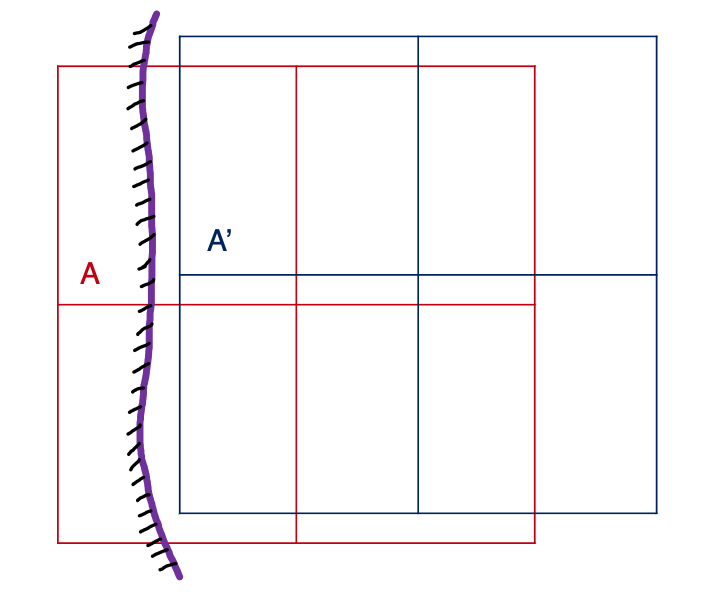
\includegraphics[width = 0.6\textwidth]{resamp_demo.png}
\caption{Illustration of subvoxel effects, caused by the ambiguous position of a structure boundary within a voxel before and after resampling. Due to the application of some transformation, the voxel grid shifts from red to blue; voxel $A$ becomes voxel $A'$. A structure boundary is shown in purple, with the dashed side as the interior, so voxel $A$ is approximately 30\% interior and 70\% exterior. After resampling, $A'$ overlaps significantly with $A$, so will be assigned a similar value to it, even though it does \textit{not} intersect the structure at all. This arises due to the assumption of uniform signal distribution within voxels, which is anatomically incorrect.}
\label{resamp_demo}
\end{figure}

The voxel labelled $A$ is transformed to $A'$. Prior to transformation, voxel $A$ contains PVs caused by the partitioning of the voxel by the structure boundary (approximately 30\% interior and 70\% exterior). The signal in voxel $A$ will therefore be a mixture of interior / exterior signals in proportion to the PVs. After application of the transformation, it is necessary to evaluate the new signal for voxel $A'$. Because of the significant overlap between voxel $A$ and $A'$, the resampled value for $A'$ will be strongly weighted towards $A$ (the exact weighting is determined by the interpolation function used; but in any case $A$ will contribute substantially). As a result, the resampled value for $A'$ will contain a non-zero proportion of signal from the interior of the structure. This is despite the fact that voxel $A'$ does not actually intersect the structure at all, so the correct solution for $A'$ would not contain any signal from the structure. 

The above situation arises due to the assumption of uniform signal distribution that is made during interpolation. The interpolated value for a voxel is evaluated as a weighted average across neighbouring voxels, where the weights are determined by the relative distances of these neighbours. Importantly, the operation is blind to the distribution of signal \textit{within} those neighbours, and specifically the fact that they may contain PVs, because there is no finer discretisation of the data available. As there is no basis for determining which signal contributions within the neighbours should or should not be included in the output, the assumption of uniform distribution is instead made, leading to an artificial increase in PVE in the output. This mechanism - the lack of information about spatial distribution of signal within a voxel - is hereafter referred to as the \textit{subvoxel effect}. A practical example of the impact of the subvoxel effect on a structural T1w image is shown in figure \ref{translate_data}. 

\begin{figure}
\centering
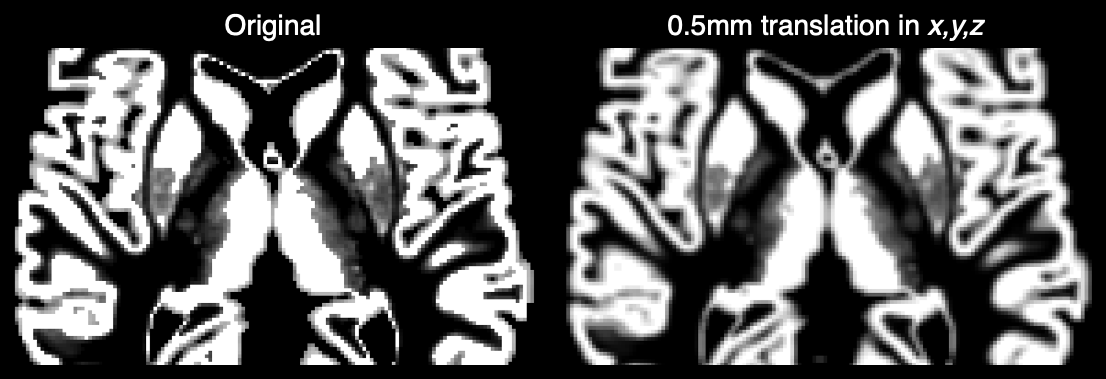
\includegraphics[width = \textwidth]{translate_data.png}
\caption{Effect of resampling on a GM PV map at 1mm resolution. The original map is shown on the left, the application of a 0.5mm translation in each axes is shown on the right. Due to the ratio of translation distance (0.5mm) to voxel size (1mm), subvoxel effects are maximised; a significant loss in edge definition is observed after resampling.}
\label{translate_data}
\end{figure}

It is difficult to quantitatively measure the impact of resampling on PVE. To do so would require the ability to express some volumetric ground truth data in an arbitrary voxel grid without making use of resampling, otherwise a trap of circular reasoning results. Such an analysis can however be performed using simulations. In particular, by using simulated surfaces to represent structure boundaries, it is possible to calculate PVs in any arbitrary grid to a high precision via a numerical method. The impact of resampling may then be quantified by performing a comparison between i) direct evaluation of PVs in an arbitrary voxel grid using the numerical method, and ii) evaluation of PVs in a high resolution voxel grid using the numerical method followed by resampling into the same arbitrary grid. For example, PVs can be obtained in a 3mm voxel grid either by direct evaluation of the numerical method in that grid, or by evaluating PVs in a 1mm grid and then resampling them to the lower resolution. Figure \ref{resamp_ratio} shows the results of such an analysis, applied to the simulated surfaces representing cortical anatomy that will be detailed later in section \ref{tob_sim_surfaces}. 

\begin{figure}
\centering
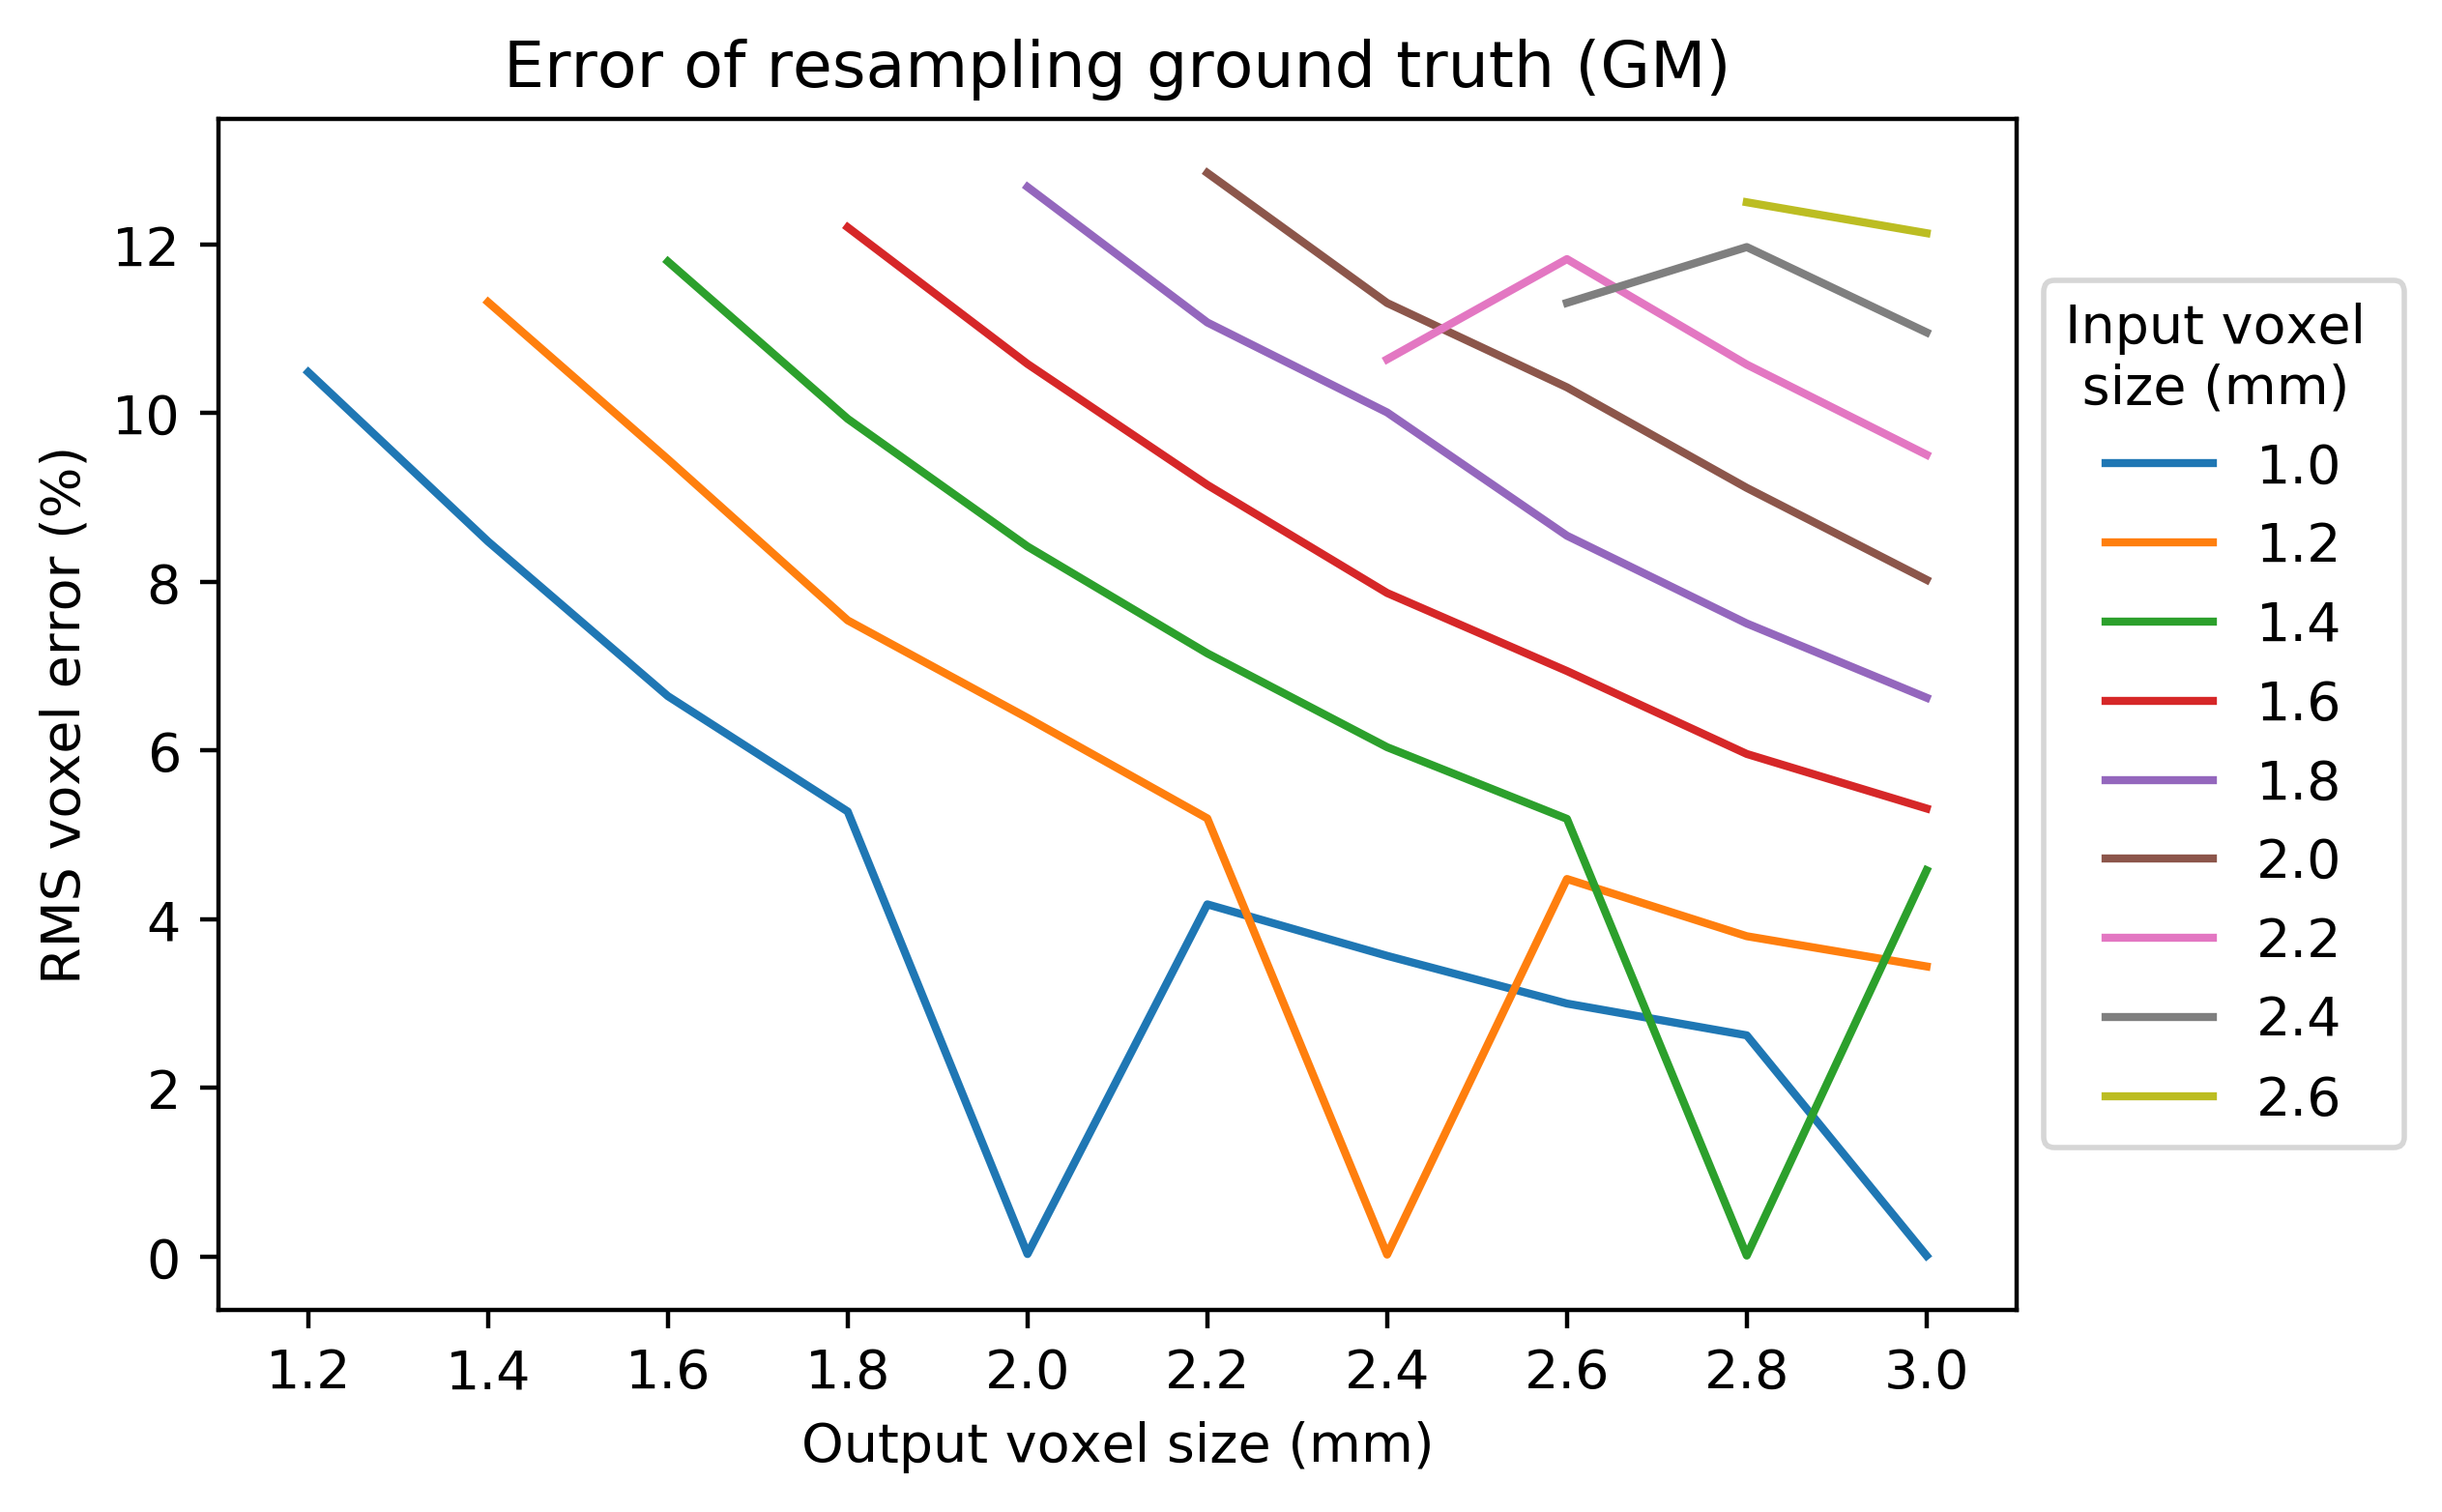
\includegraphics[width = 0.7\textwidth]{resamp_ratio.png}
\caption{Error associated with resampling a PV map as a function of input and output voxel size, masked to consider only voxels containing PVs. At each resolution, PVs were calculated either by i) direct evaluation of a numerical method, or ii) resampling the results of the numerical method \textit{from a smaller voxel size}. In general, the error due to resampling decreases as the ratio of output to input voxel size increases. When this ratio takes an integer value, the error can disappear completely, but this is due to the perfect alignment of voxel grids within this simulation.}
\label{resamp_ratio}
\end{figure}

Each trace on the plot represents a different input voxel resolution at which ground truth PVs were evaluated. These ground truth maps were then resampled to all resolutions above the input (for example, the 1.4mm truth was resampled to 1.6, 1.8, ... \textit{etc}), and the root mean square (RMS) voxel error with respect to ground truth evaluated (masked to consider only voxels that contain PVs on the ground truth). Multiple trends were seen: firstly, as the input voxel size increased, error at all output voxel sizes increased. Secondly, as the ratio of output to input voxel size increased, the error decreased. Finally, the error fell to zero when this ratio took an integer value. This was due to the use of perfectly aligned voxel grids for these simulations, which in turn meant that each large voxel corresponded perfectly to a grid of $N$ smaller voxels on the input data (where $N$ is the ratio of voxel sizes). The significance of an integer ratio of voxel size is that subvoxel effects are eliminated: the input voxel is entirely contained within a single output voxel, so the assumption of uniform signal distribution is of no consequence. Hence, this analysis demonstrates that resampling has the effect of further mixing, or increasing, whatever PVE may already be embedded within data. 


\subsection{Implications for PVEc} 

Given that resampling further increases the PVE embedded within data, it is logical to question whether this will have implications for the successful application of PVEc. This is especially pertinent for analysis strategies that do not operate in native acquisition space. For example, the analysis paradigm adopted by some SPM (a neuroimaging software package) and HCP pipelines places an emphasis on the immediate transformation of raw data into MNI space, though it is important to note that PVE are less of a challenge for the modality these pipelines are designed for (BOLD) \cite{Glasser2013, Friston2003a}. 

This question also applies to the analysis of repeated acquisitions of the same subject. A frequently cited theoretical justification for PVEc is that it can improve the repeatability of parameter measurements by removing the dependence of voxelwise measurements on tissue PV. This is necessary because PVs are acquisition-specific, arising due to the particular interaction of subject anatomy with an imaging matrix at the exact moment of acquisition. Due to subject motion, for example, the embedding of PVE across repeats cannot therefore be assumed to be constant. 

This poses a challenge for any analysis that requires spatial correspondence across repeats. Consider, for example, co-registration of repeat ASL data into alignment with a structural image at original voxel resolution. Assuming perfect registration and constant perfusion across the repeats, signal from any given location within the brain should in theory end up in the same voxel in common analysis space, and therefore that voxel should have the same value across all repeats. In practice, the PVE that were embedded within the repeat data were different, and therefore this voxel in common space will have different values across the repeats. The justification for performing PVEc is immediately clear; removing the differing embeddings of PVE within the repeat data should reduce variability of measurements between repeats. The challenge is in determining \textit{what} PV estimates should be used for the correction. 

The obvious approach would be to use PV estimates obtained from a segmentation of the structural image. This is made simpler by the fact that the common analysis space is already in alignment with the structural image, so all that is required is a downsampling with identity transformation of the PV estimates in the structural grid to the ASL grid. The schematic for such a strategy is illustrated in figure \ref{rpt_paradox} and is hereafter referred to as the \textit{naive} approach. Nevertheless, this approach is somewhat paradoxical: \textit{one} single set of PV estimates are used to correct \textit{all} of the repeat data, despite the fact that the PVE within each are expected to be different. It therefore follows that this strategy for PVEc will lead to sub-optimal outcomes. 

\begin{figure}
\centering
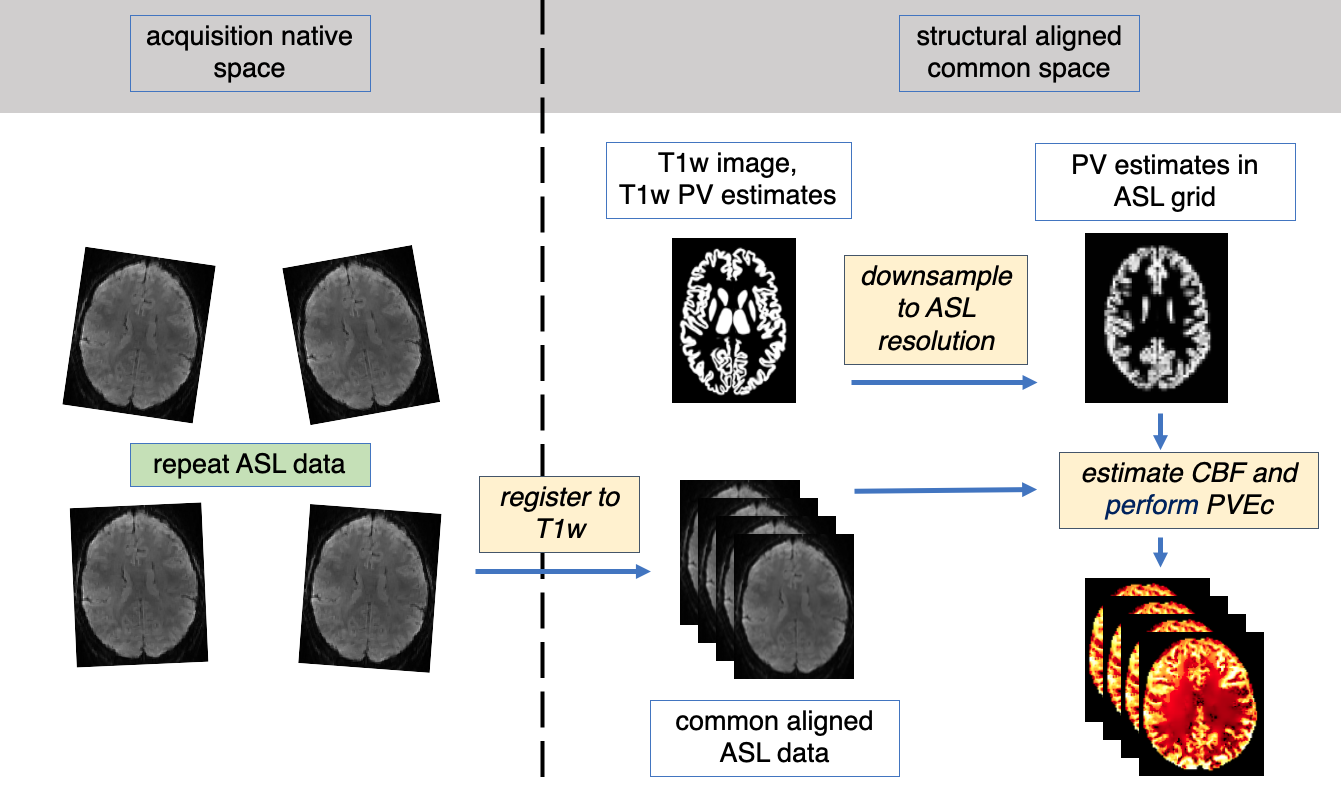
\includegraphics[width = \textwidth]{rpt_paradox.png}
\caption{The paradox of PVEc in a common analysis space for repeat data. The point of origin is highlighted in green. The ASL repeats are co-registered into a common analysis space, and then PVEc is performed using a single set of PV estimates downsampled from structural resolution for all repeats. This is despite the fact that theoretical understanding of PVE suggests each individual repeat will contain \textit{different} PVE.}
\label{rpt_paradox}
\end{figure}

What is instead required are a set of PV estimates for each repeat that convey information about the PVE that held true \textit{at the time the data was acquired}. These can readily be obtained by reversing the transformation between the native ASL data and the structural image, so that the T1w PV estimates are transformed and downsampled into the native voxel grid of the ASL data. Thereafter, the same set of transformation operations that are required to move the repeat data into common space are simultaneously applied to the native space PV estimates. This means that whatever extra PVE are introduced into the data by resampling are also introduced into the PV estimates themselves. In effect, the PVs that held true at the time of acquisition are updated to incorporate the extra PVE that are introduced by resampling. Because this strategy involves the use of two resampling operations for the PV estimates (firstly, from structural space to ASL native space, and then from ASL space to the common analysis space), this strategy is referred to as the \textit{double-resampling} approach, the schematic of which is illustrated in figure \ref{dbl_paradox}. The amount of PVE introduced by the two resampling operations will be very different. The resampling from structural to native ASL space introduces little PVE (subvoxel effects are minimal because the ratio of output to input voxel size is greater than unity), whereas the resampling from native ASL space to the common analysis space introduces high PVE (the ratio of output to input voxel size is unity). 

\begin{figure}
\centering
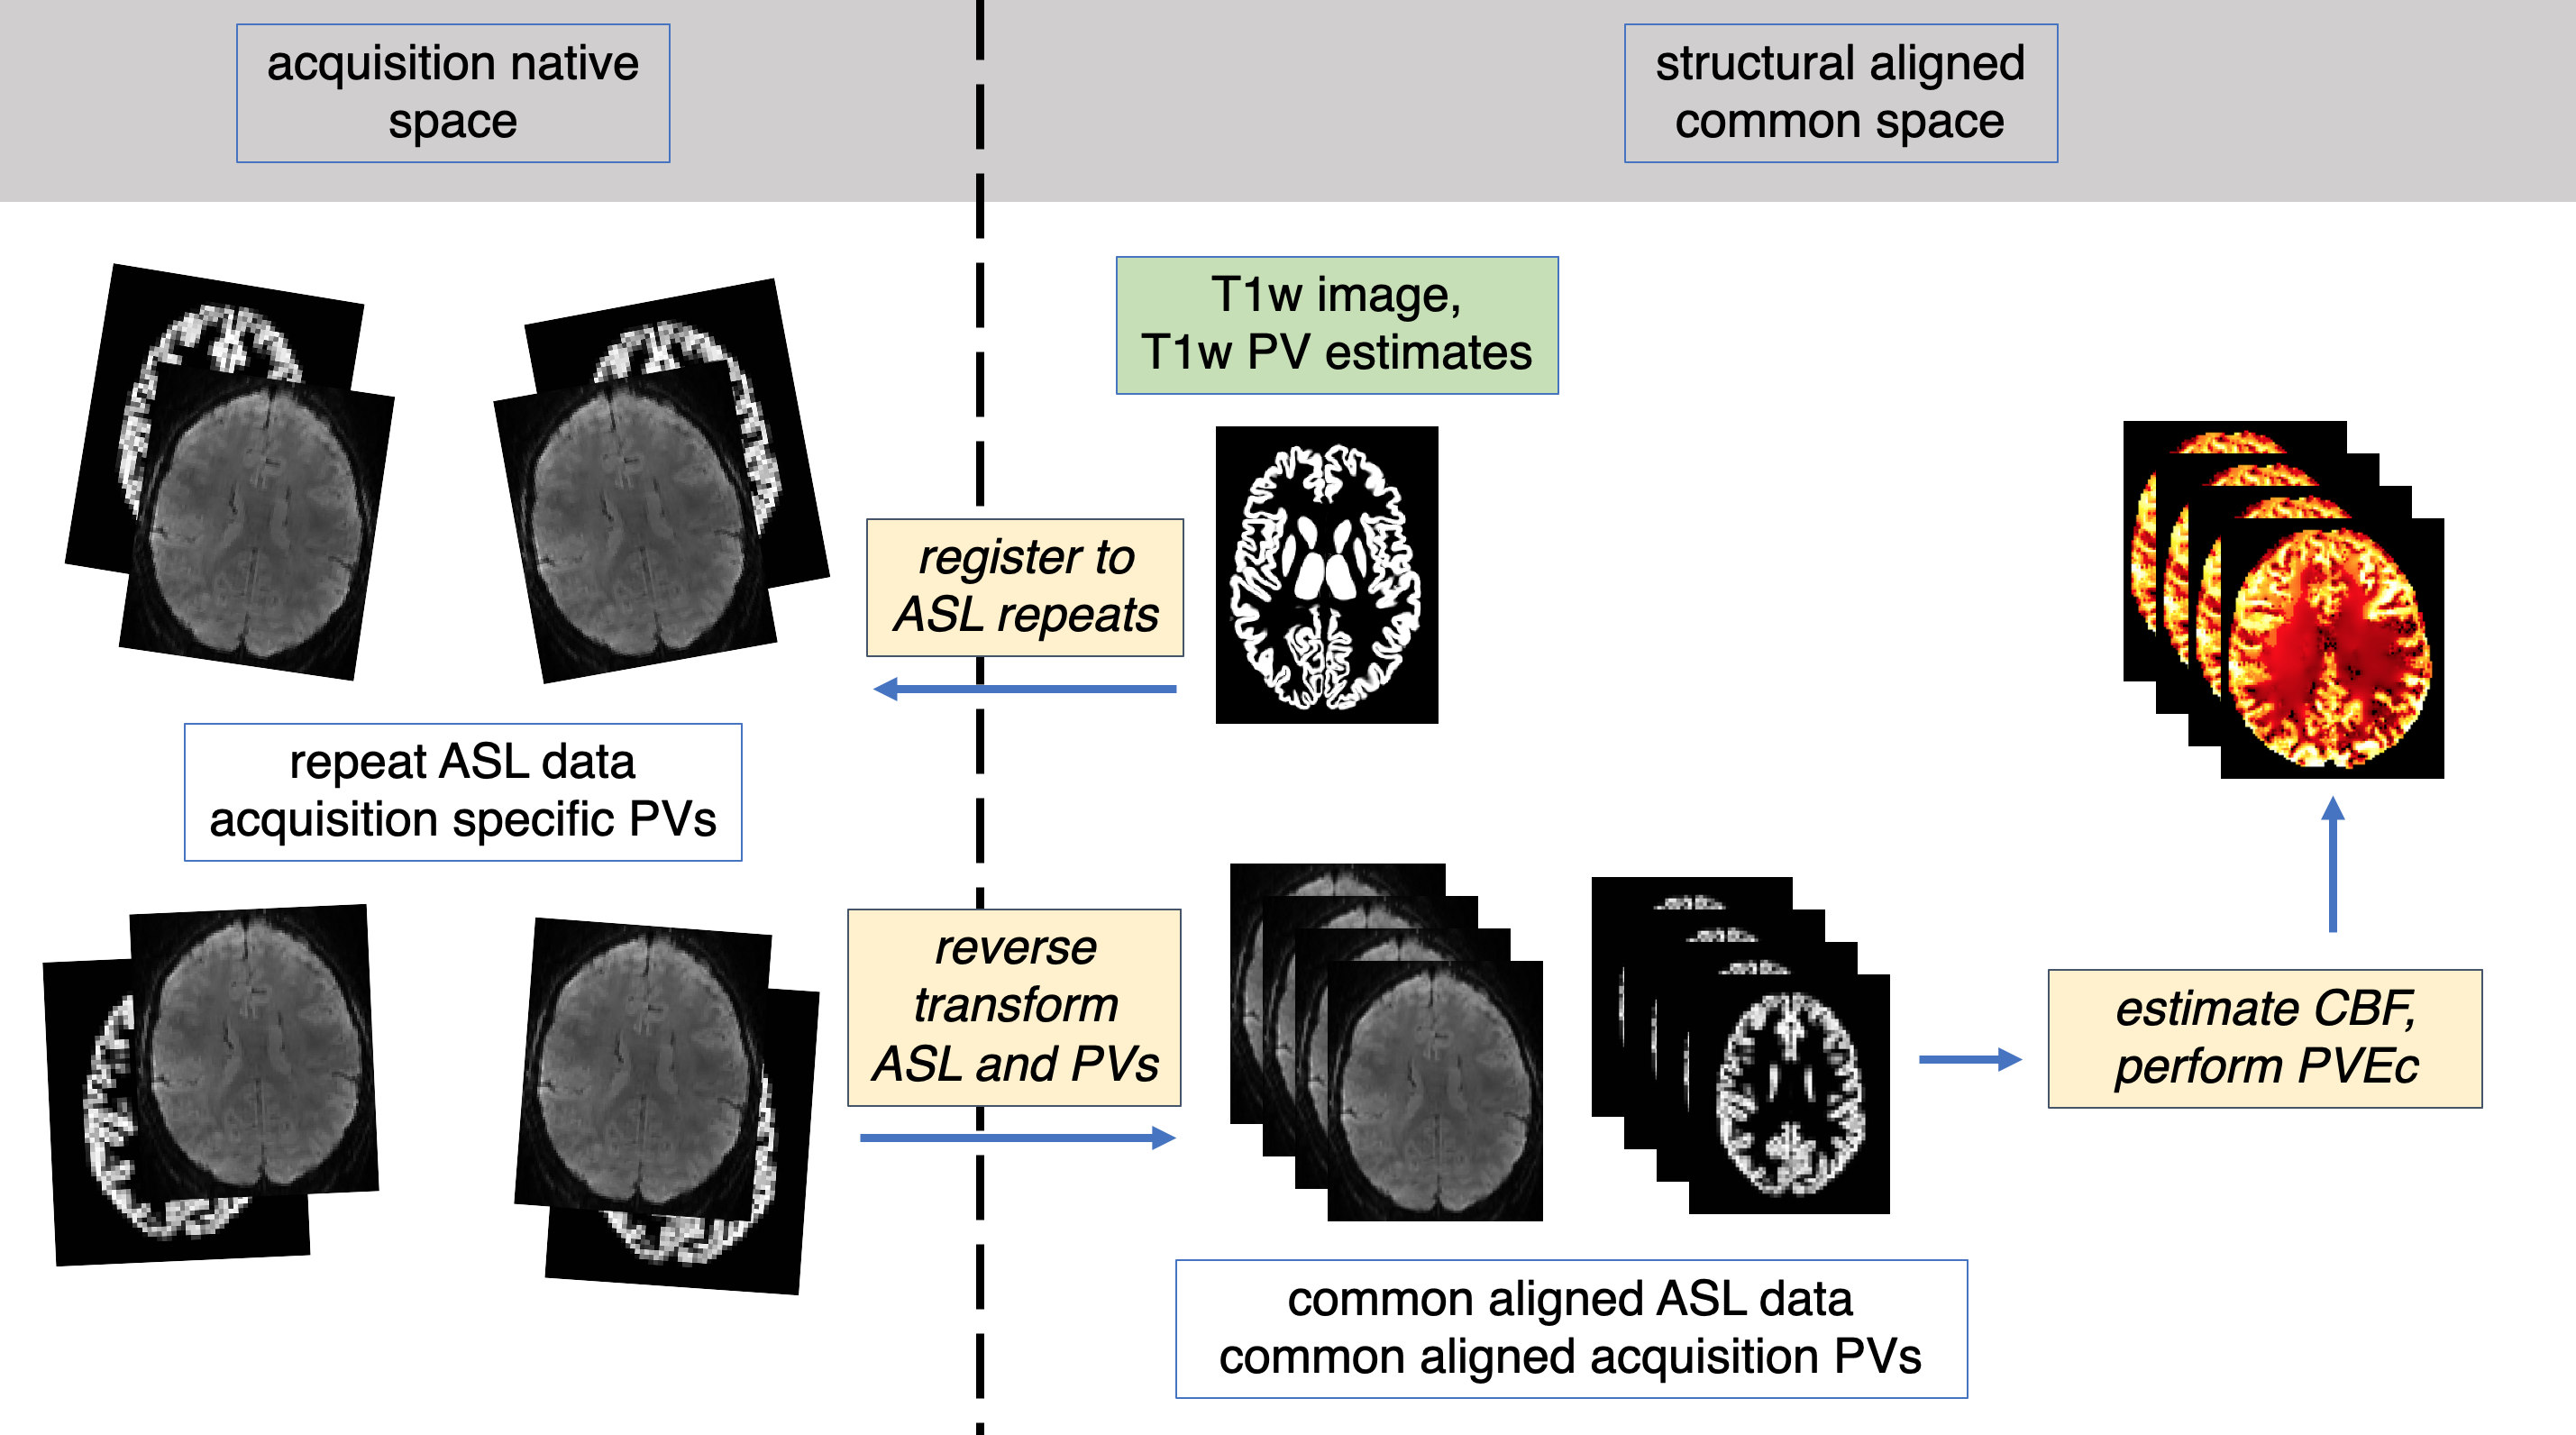
\includegraphics[width = \textwidth]{dbl_paradox.png}
\caption{The double-resampling strategy for PVEc of repeat data in a common analysis space. The point of departure is highlighted in green. PVs are first estimated in the native space of each repeat acquisition, and then undergo the same set of transformations into common space. This results in a unique PV map used for the correction of each repeat in common space, which better matches theoretical understanding of the origin of PVE.}
\label{dbl_paradox}
\end{figure} 


\subsection{Experimental hypothesis}
The hypothesis investigated in this chapter is that the consequences of resampling are substantial enough to negatively impact the application of PVEc. The corollary of this is that, if PVE are to be minimised, analysis in the native space of the data should always be preferred (though there may of course be other reasons to perform analysis in a non-native space). Finally, it is hypothesised that if estimation in a non-native space is required, then the double-resampling strategy for obtaining PV estimates outperforms the naive strategy. These hypotheses have been investigated using simulated and \textit{in-vivo} ASL data. 

\section{Datasets}

\subsection{Terminology}

The following terminology is hereafter used. \textit{Original, acquisition} or \textit{native} space data refers to ASL data in the same voxel grid and alignment as that in which it was simulated or acquired; \textit{i.e.}, data that has not been processed in any way. \textit{Resampled} data refers to data that has been through a resampling process, potentially involving a transformation into different alignment, and \textit{common space} data refers to data has been transformed and resampled into alignment with some external reference for the purpose of establishing spatial correspondence between repeat acquisitions. For all the analyses presented herein, \textit{common space} was defined in alignment with the subject's anatomical image at the same voxel size as the native ASL data. 

PVEc was always performed with partial volume estimates that were in alignment with the ASL data. The only variable in the process was the amount of resampling that had been applied to the PV estimates: \textit{naive} refers to PV estimates obtained via the shortest possible path (\textit{e.g.}, direct downsampling from structural resolution), whereas \textit{resampled} refers to naive estimates that have been through the same set of resampling operations as the ASL data itself. Finally, in the context of repeat data in a common analysis space only, \textit{double-resampled} means naive PVs that have been transformed into the acquisition space of the ASL data, and then reverse-transformed back into the common analysis space alongside the ASL data itself. This is a round-trip transformation resulting in no change in the alignment of the PV estimates themselves, but extra PVE will be introduced due to the resampling operations. 

\subsection{Simulated data}
\label{pvec_chapter_sim_data}

Simulated ASL data was produced using structural pre-processed data for subject 103818 from the HCP \cite{Glasser2013}. Surface segmentations of the cortex and subcortex for this subject were processed to yield a reference set of PV estimates using the surface-based method detailed in chapter \ref{tob_pv_chapter}. The ASL signal was calculated using the \textit{aslrest} model included with FSL FABBER \cite{Chappell2009} for pure GM and WM respectively and then combined in linear proportion using the PV estimates. As FABBER was also used for perfusion estimation, this implies that in the idealised case it should be possible to perfectly recover ground truth parameter values from the simulated data. The simplifying assumption of constant CBF and ATT in both GM and WM was made. Typical values of 60, 20 ml/100g$\cdot$min and 1.3, 1.6s were used for GM and WM respectively. The assumption of constant CBF and ATT is helpful because it means that any within-tissue variance in the data must be explained by PVE, which in turn means the efficacy of PVEc can be assessed by observing reductions in within-tissue variance of the output parameter distributions. Other simulation parameters were as follows: pcASL of 1.8s label duration with 5 PLDs (0.75, 1.0, 1.25, 1.5, 1.75, and 2.0s) and 8 repeats at each PLD (a total of 48 label-control pairs). 

One timeseries was simulated with high SNR in order to provide an insight into the PVE/resampling interaction in the absence of `real-world' confounds. SNR was defined via 

\begin{equation}
\label{snr_defn}
\mathrm{SNR} = \frac{s \sqrt(n)}{\sigma}
\end{equation}

where $s$ represents maximum signal in pure GM, $n$ is the number of volumes in the timeseries, and $\sigma$ is the standard deviation of noise. When applying this relation to \textit{in-vivo} data, $s$ may be approximated by taking the maximum timeseries-mean of the data. With the aforementioned sequence parameters, $s$ was 45 arbitrary units (a.u.) at 1.5s PLD. Zero-mean white noise was added to the data to yield an SNR of 27. 

Four repeat timeseries were simulated with low SNR to realistically model the challenges of working with \textit{in-vivo} data. Using the same definition of SNR and maximum signal value (45 a.u. at 1.5s PLD), zero-mean white noise was added to the data to yield an SNR of 9. In order to simulate the effects of patient motion during a scanner session, the low SNR repeats were each produced in their own `acquisition-specific' alignment. This was achieved by applying four random affine transformations to the reference PV estimates to produce acquisition-specific PV maps, from which the ASL data was simulated. Finally, the reverse transforms were applied to the ASL data to bring them back into alignment with the reference PV estimates in common space. The transformations were generated by concatenating rotations around the $z$ and $x$ axis with a translation along each axis; the rotations were drawn from the uniform integer distribution between [0, 5] degrees and the translation components in $xyz$ were drawn from the uniform continuous distribution between [0, 6]mm. This process is illustrated in figure \ref{simrpt_schema}. 

\subsection{\textit{In-vivo} data}

\textit{In-vivo} data was acquired for two subjects at 7T using a single TI pASL sequence. For the first subject, one timeseries of 200 volumes was obtained (referred to as the `high SNR' data); for the second subject, three timeseries of 100 volumes were obtained in the same session (referred to as the `low SNR repeats'). Other sequence parameters were as follows: QUIPSS-II labelling of 700ms bolus duration, 1.8s TI, 1.5mm isotropic voxel size on an imaging matrix of 128 x 128 x 36 and 2D EPI readout with 0.0325s slice acquisition time. The data was then downsampled without interpolation to 3mm isotropic voxel size by summing over 2x2x2 voxel grids to increase PVE and improve SNR. Using the definition of SNR given in equation \ref{snr_defn}, the SNR of the repeats after this processing was estimated to be around 9. 

Structural T1w MP2RAGE images were obtained at 0.7mm isotropic resolution for both subjects and processed using FreeSurfer and FSL FIRST to obtain surface segmentations. The surface-based method detailed in chapter \ref{tob_pv_chapter} was then used on these to obtain PV estimates. All registration between ASL and structural data was performed using FSL FLIRT (including MCFLRIT for motion correction) with six degrees of freedom \cite{flirt}. 

\section{Methods}

\subsection{Perfusion quantification and PVEc}

Two forms of PVEc were investigated: Asllani's LR method \cite{Asllani2008} and the spatially regularised mode incorporated within BASIL \cite{Chappell2009, Chappell2011}. The LR method can be applied to either ASL data itself, or uncorrected  CBF and ATT maps resulting from a non-PVEc run. The former variant (`LR on data') was used for this work as it better preserves the differing dynamics of perfusion for each tissue with multi-PLD data. This was achieved by performing the regression on each volume of the ASL timeseries to yield two separate timeseries for GM and WM. FSL BASIL was then run on each output timeseries independently in non-PVEc mode (with tissue properties fixed for GM or WM as appropriate). A 3x3x3 kernel including cardinal neighbours only (a total of six neighbours per voxel) was used. It is well-documented that the LR method provides a relatively high and fixed level of smoothing to data, but the extent of smoothing does not depend on the data itself (and is fixed instead by the kernel size). 

The spatially-regularised PVEc built into BASIL is conceptually similar to the LR approach in that it also uses a kernel of neighbouring voxels in order to separate signal into GM and WM contributions. The key difference is that the weight given to the kernel (the spatial precision) is a parameter of the VB inference process that is optimised; it therefore provides adaptive spatial smoothing in a data-driven manner that has been shown to better preserve details than the LR method \cite{Zhao2017a}. A crucially important aspect of spatially-regularised BASIL is that it makes use of a Laplacian spatial prior to condition the under-determined system of equations that arise due to PVE in each voxel neighbourhood. It \textit{also} makes use of the spatial prior as a means of mitigating the low SNR commonly seen in ASL data. This dual use of the spatial prior - as a means of reducing noise, and as a means of implementing PVEc - means it is difficult to quantitatively compare the amount of smoothing that it deems optimal across different datasets, or that it deems optimal for PVEc versus non-PVEc. This is in contrast to the LR method for which the amount of smoothing is a fixed property of the regression kernel.

For both variants of PVEc on simulated data, both CBF and ATT were estimated. All tissue and model properties were left at their default BASIL values (the same used when simulating the data). 

For the \textit{in-vivo} data, the following BASIL settings were used to estimate CBF only (both variants of PVEc were used). ATT was fixed at the reference value of 1.3s or 1.6s for GM and WM respectively, the T1 value of blood at 7T was set at 2.1s and the pASL labelling efficiency was set at 0.95 \cite{Zhang2013}. Slice time correction of 0.065s was used and the calibration was performed in a voxelwise manner. 

All transformation, resampling and interpolation operations were performed using the \textit{regtricks} software package \cite{regtricks} with trilinear interpolation and intermediate supersampling (the same approach used by FSL \textit{applywarp}). Although other interpolating basis functions can reduce the loss in spatial resolution associated with resampling, trilinear interpolation remains in very common usage, particularly for low resolution data. 

\subsection{Simulated data}
\label{pvec_simulation_data_section}

In order to investigate the effect of resampling on PVE in the absence of any other effects, the high SNR data was taken through a round-trip of resampling. A random affine transformation (generated in the same manner as for the simulated repeats) was applied to the data to forward-transform it, followed by a separate application of the reverse transform. This resulted in data that had been through two rounds of resampling but remained in its original alignment. The PV estimates were also taken through the same round-trip, CBF was estimated from both the original and resampled data, and finally PVEc was performed using both the naive (original) and resampled PV estimates. The schematic for this is illustrated in figure \ref{doublesim_schema}. 

\begin{figure}[h]
\centering
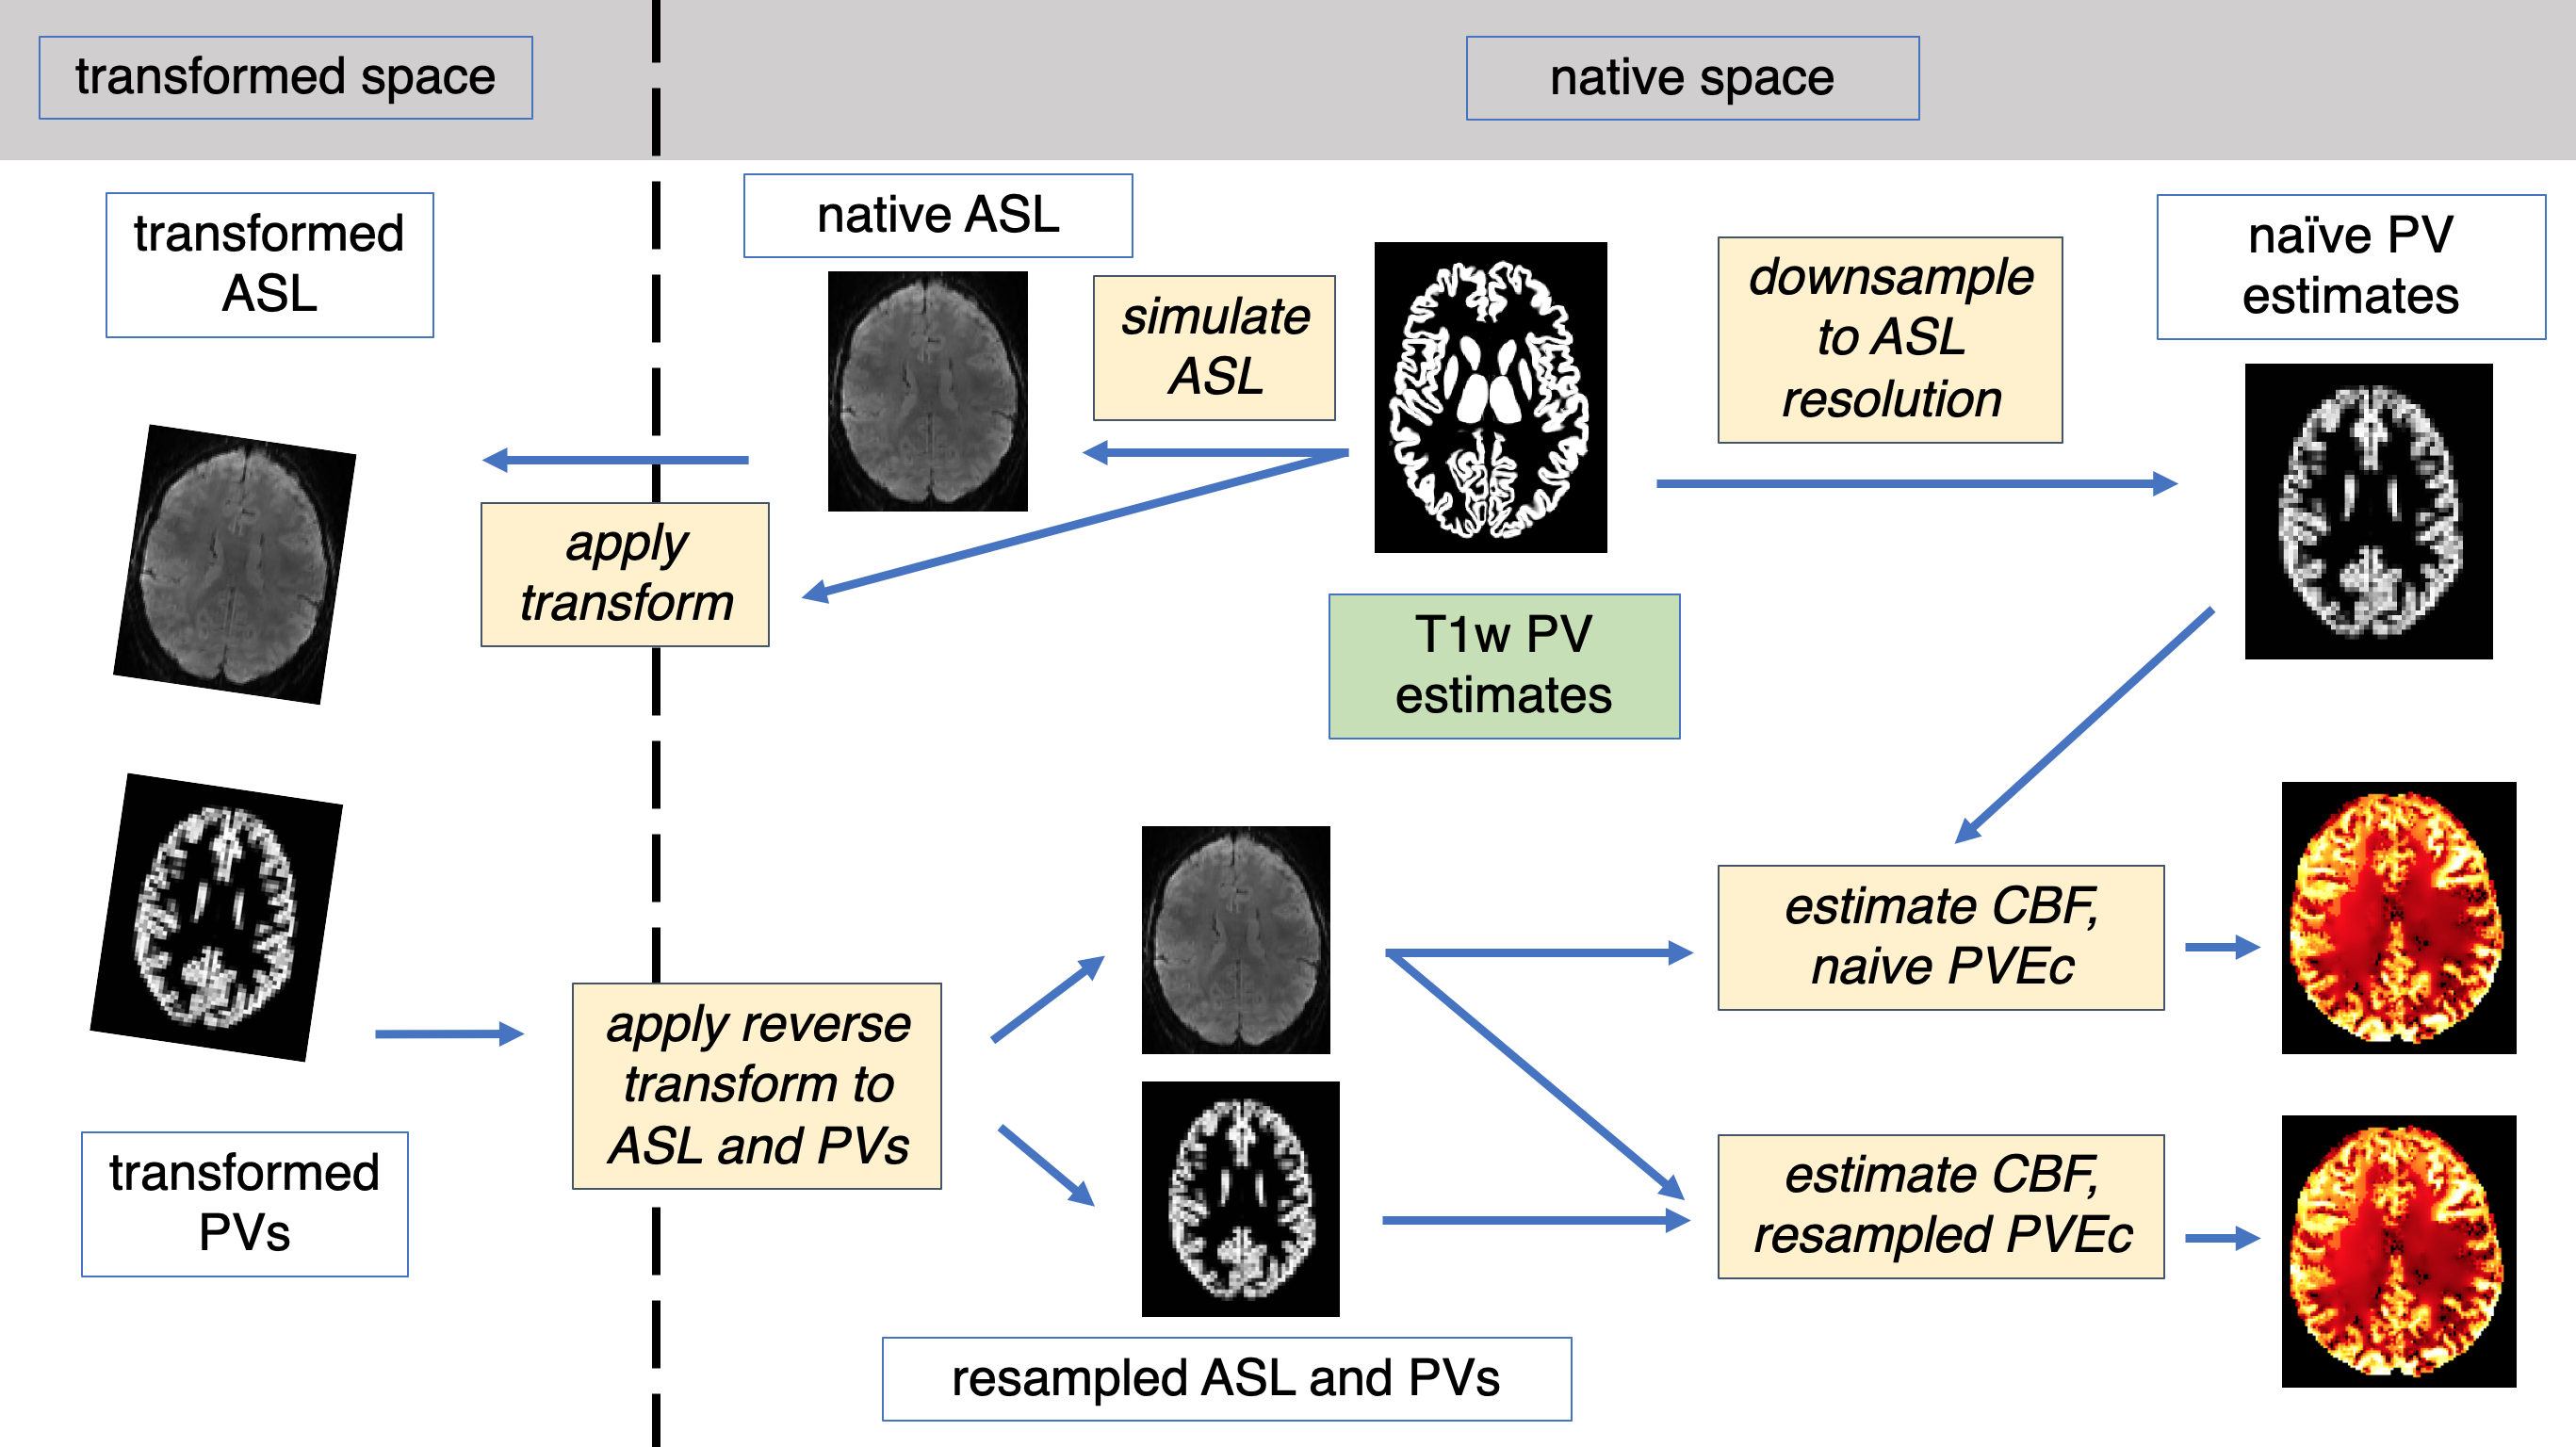
\includegraphics[width = \textwidth]{doublesim_schema.png}
\caption{Schematic of simulation and round-trip transformation for the high SNR simulation data. The point of departure is highlighted in green. ASL data was generated in alignment with the anatomical ground truth PV estimates, and then underwent a round-trip of transformation, alongside the PV estimates. Finally, the transformed ASL data was corrected with both the original PV estimates (naive) and the transformed PV estimates (resampled), and a comparison made with the original data corrected with original PVs (not shown).}
\label{doublesim_schema}
\end{figure}

The extent of PVE within the data was evaluated by drawing histograms of uncorrected voxelwise CBF. The efficacy of PVEc was determined by plotting the distribution of CBF for each tissue after correction; in the ideal case two sharp peaks at 60 and 20 units would be observed for GM and WM respectively. PVEc CBF maps for each tissue were masked to include voxels with at least 5\% of that tissue on the reference (\textit{i.e.}, naive) set of PV estimates. This masking step was necessary because BASIL's PVEc implementation returns tissue CBF estimates for all voxels, including those that do not actually contain the tissue of interest. The strength of the PVE mechanism was evaluated by performing linear regressions of uncorrected CBF against GM PV; theory predicts that CBF should be directly proportional to tissue PV. 

In order to investigate the consequences of transforming repeat data into a common analysis space, simulated ASL repeats were analysed using the schematic given in figure \ref{simrpt_schema}. CBF estimation and PVEc were performed in common space using naive and double-resampled PV estimates. Coefficient of variation (CoV) across the repeats was evaluated in a voxelwise manner by dividing the standard deviation of CBF estimate by the mean. CoV was then averaged within ROIs defined according to GM PV thresholds on the naive set of PV estimates (eight bins of 10\% width, from 20 to 100\% GM PV). This definition of ROI was made purely as a means of establishing spatial correspondence between voxels of the repeated runs, and did \textit{not} genuinely reflect the PVE that are present within each of the runs (which are expected to be different, the very premise of the double-resampled strategy). PVEc CBF maps for each tissue were masked to consider voxels with at least 5\% of the tissue in question. As a final comparator, the individual repeats were also analysed with PVEc in their respective native spaces, and the resultant corrected CBF maps were transformed into the common analysis space. CoV was then calculated in the same manner. This strategy is referred to as `BASIL [or LR] resample after PVEc' and is consistent with the principles of performing all parameter estimation in acquisition-native space and only transforming the outputs.

\begin{figure}[h]
\centering
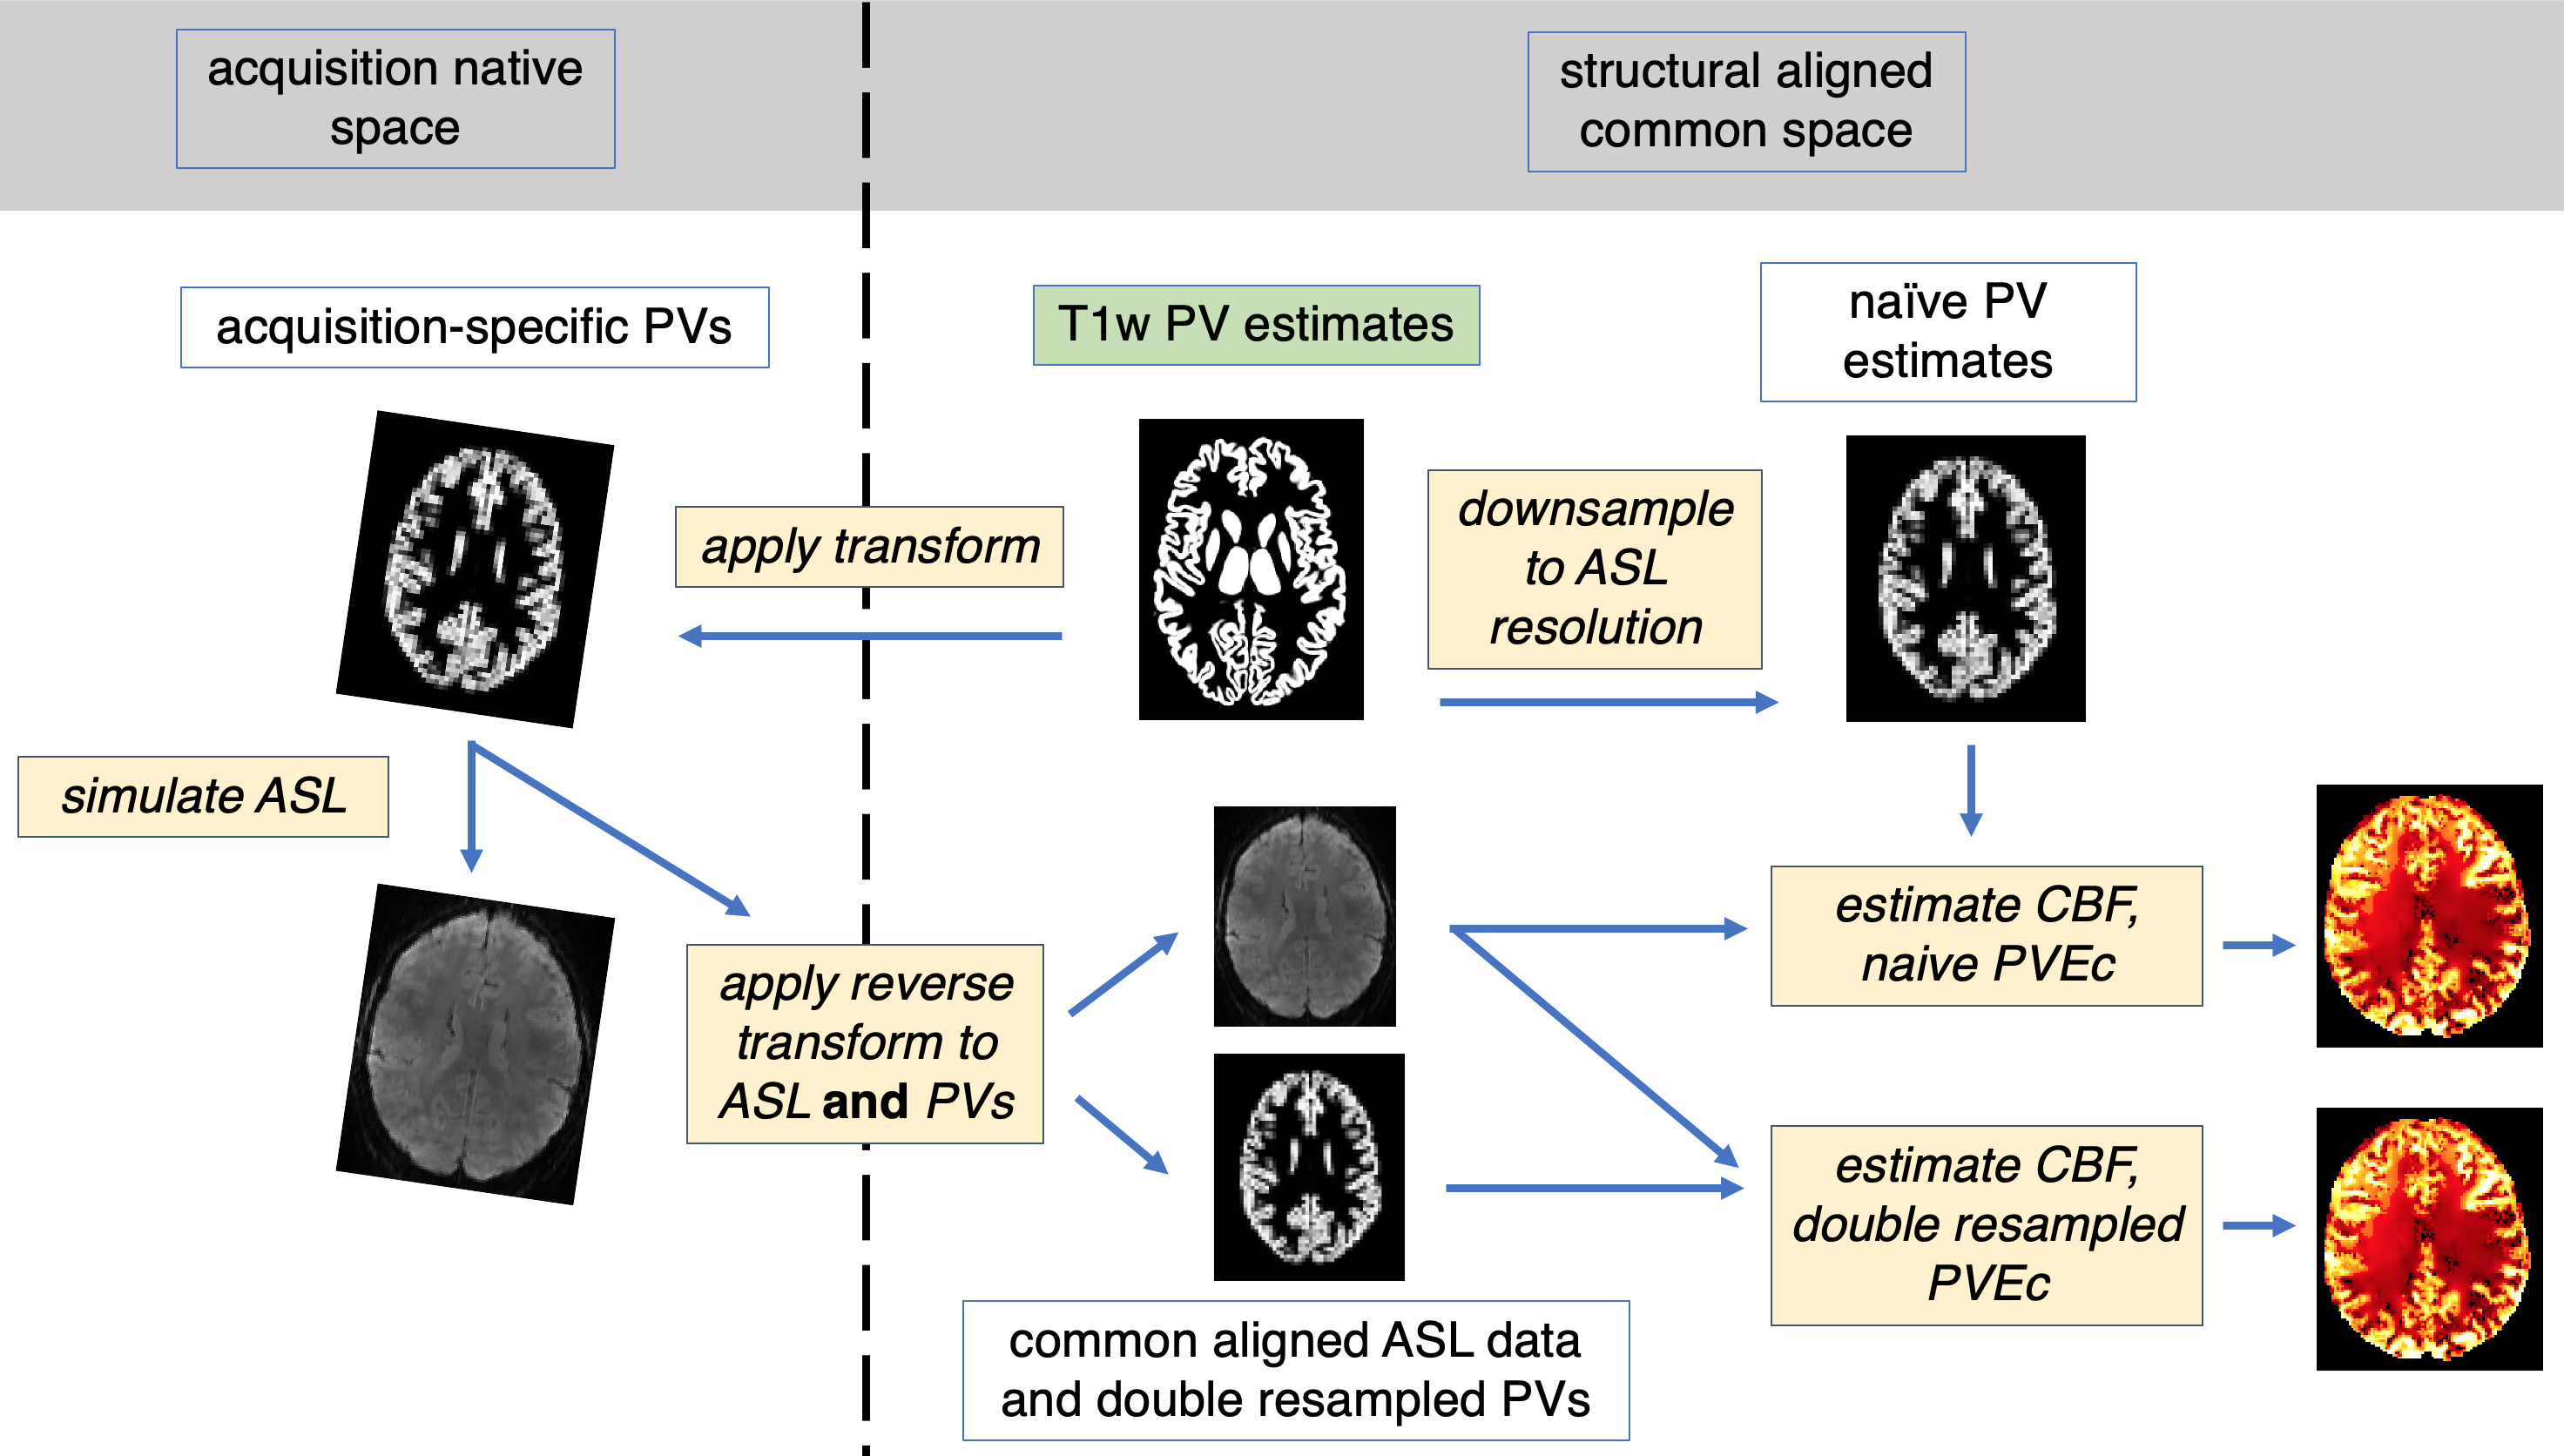
\includegraphics[width = \textwidth]{simrpt_schema.png}
\caption{Schematic of the simulated repeat ASL generation and analysis in common space. The point of departure is highlighted in green. Random transformations were applied to the ground truth PV estimates to yield a unique set of acquisition-specific PVs for each repeat, from which ASL data was then generated. Both the acquisition-specific PVs and ASL data were than transformed back into common space. PVEc of each repeat was performed using both the original PV estimates (naive) and transformed (double-resampled) estimates. As a comparator, PVEc of each repeat was also performed in native space and then the corrected output maps transformed into common space (not shown).}
\label{simrpt_schema}
\end{figure}

\subsection{\textit{In-vivo} data}

The objective of analysis on the \textit{in-vivo} data was to confirm the findings of the simulation experiments. Accordingly, the high SNR ASL data was taken through a round-trip of two resampling operations (using a transformation generated in the same manner as for the simulated repeats). PV estimates were obtained using in the native space of the ASL data the surface-based approach introduced in chapter \ref{tob_pv_chapter}, which then underwent the same set of resampling operations to yield resampled PV estimates. PVEc of the resampled ASL data was then performed using the original and resampled PV estimates. PVEc CBF maps for each tissue were masked to consider voxels with at least 5\% of the tissue in question (as was also the case for the low SNR repeat data). 

The low SNR repeats were analysed in a common analysis space in alignment with the structural image at ASL resolution. CBF estimation and PVEc were performed using both naive and double-resampled PV estimates. The schematic for these strategies was previously set out in figures \ref{rpt_paradox} and \ref{dbl_paradox} respectively. CoV was evaluated in the same manner as for the simulated repeats and ROIs were defined using the same GM PV thresholds on the naive set of PV estimates. As a final comparator, the repeats were also analysed with PVEc in their respective acquisition-native spaces followed by transformation of the output maps into the common space; this strategy is again referred to as `BASIL [or LR] resample after PVEc'. 

\section{Results}

\subsection{Simulated data}

\subsubsection{High SNR data}

\begin{figure}[H]
\centering
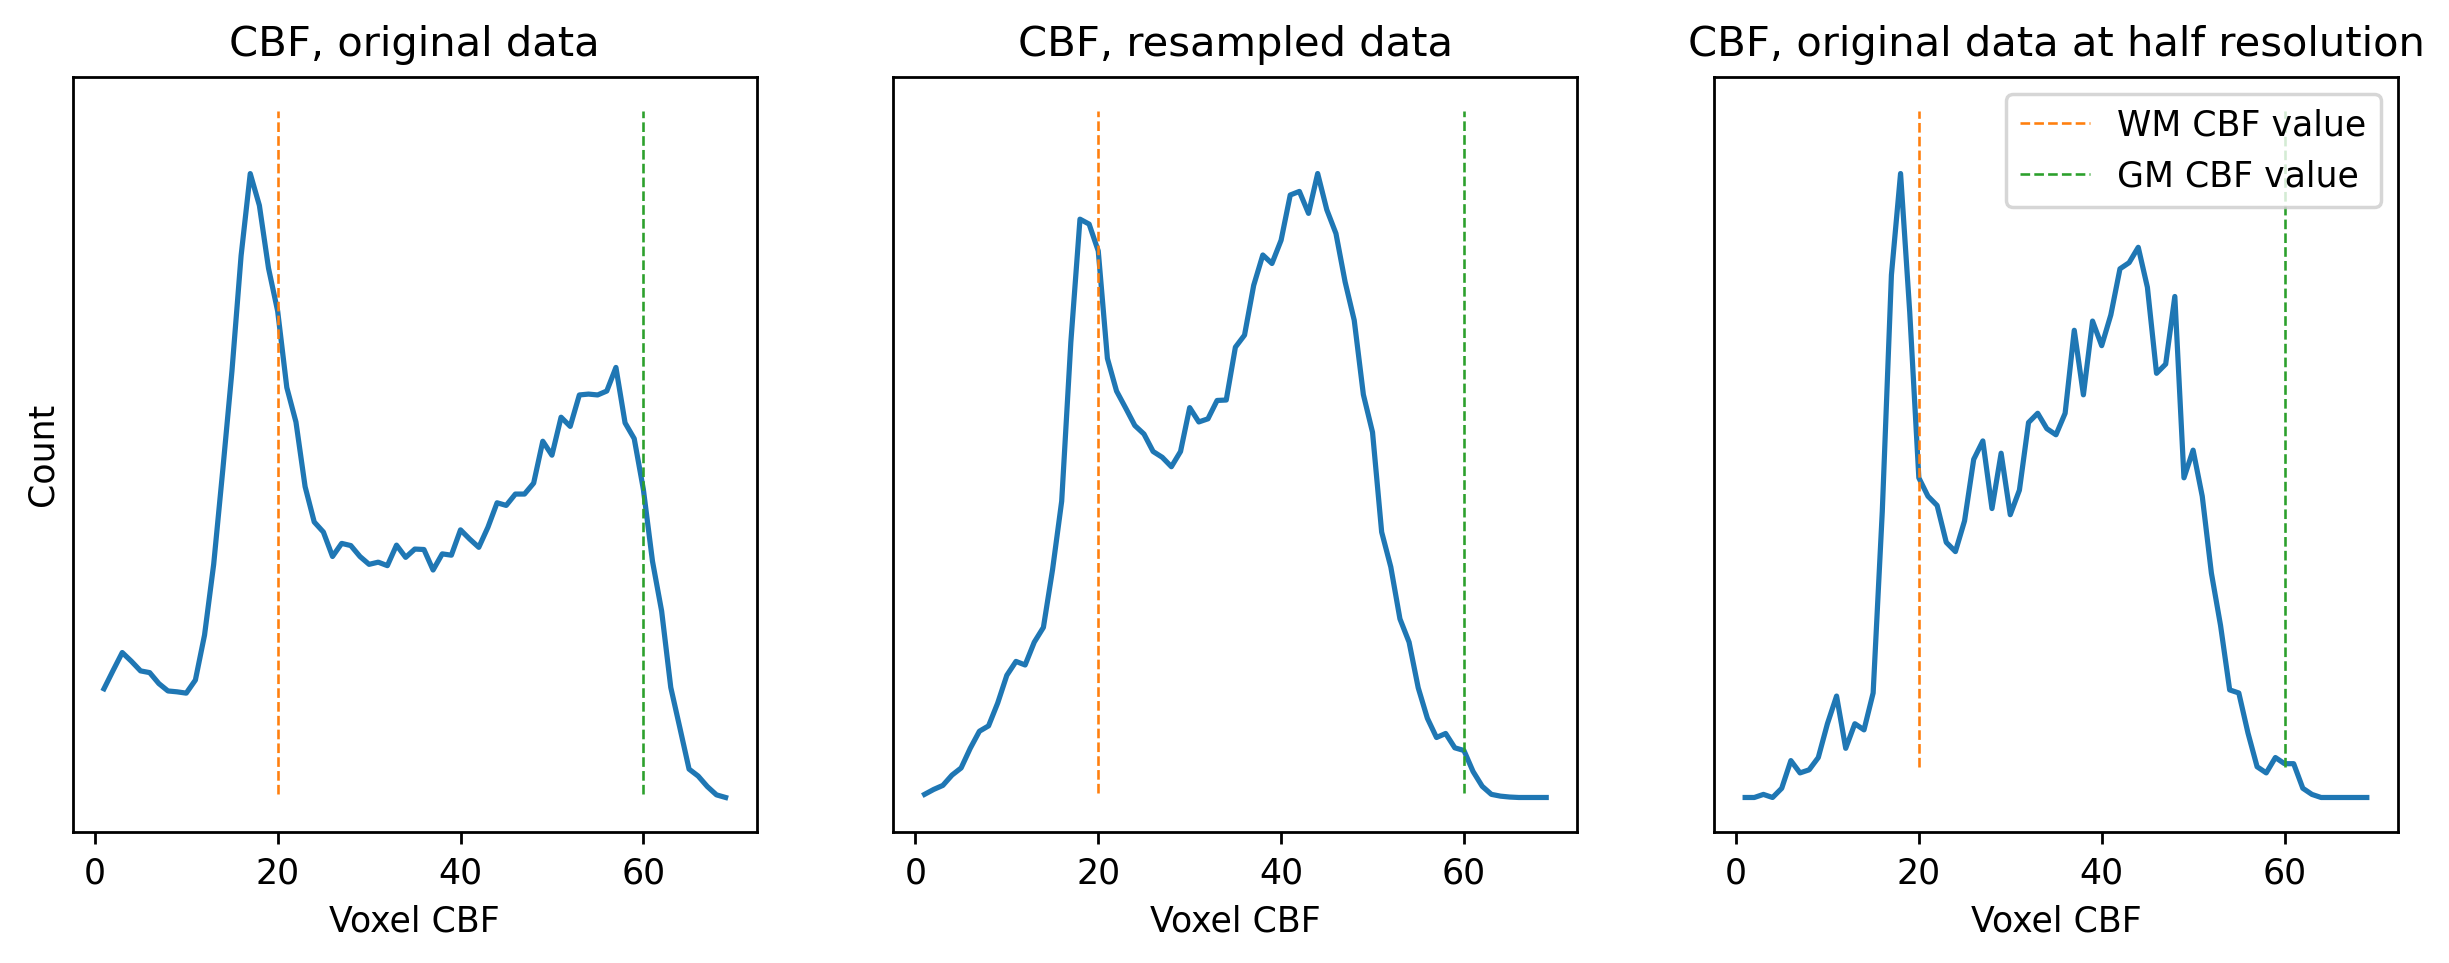
\includegraphics[width = \textwidth]{sim_asl_resamp_hist.png}
\caption{Effect of resampling on PVE within data (all plots show uncorrected CBF). Left: in the base case, CBF from the original data had a bimodal distribution with peaks corresponding to GM and WM CBF values; the extent of PVE is reflected in the large number of voxels that lie in between. Centre: CBF from the resampled data shows convergence of the distribution modes, particularly for the GM peak; this reflects an increase in PVE. Right: CBF from the original data at half the spatial resolution shows many similarities to the resampled case, demonstrating that resampling leads to an increase in PVE that would otherwise be obtained by reducing spatial resolution.}
\label{sim_asl_resamp_hist}
\end{figure}

Figure \ref{sim_asl_resamp_hist} shows histograms of uncorrected CBF estimated from the high SNR simulation data before and after resampling. The distribution of CBF on the original data was bimodal, with peaks corresponding to the ground truth WM and CBF values respectively; the presence of PVE was readily observed in the large number of voxels that lie in between these modes. After a round-trip of resampling there was a clear convergence between the modes of the distribution (in particular, the peak corresponding to GM shifted from around 60 to 40 units), indicating an increase in PVE. This change was consistent with what would be obtained if one had estimated CBF from the original data at half the spatial resolution (which is shown in the final plot). 

\begin{figure}[H]
\centering
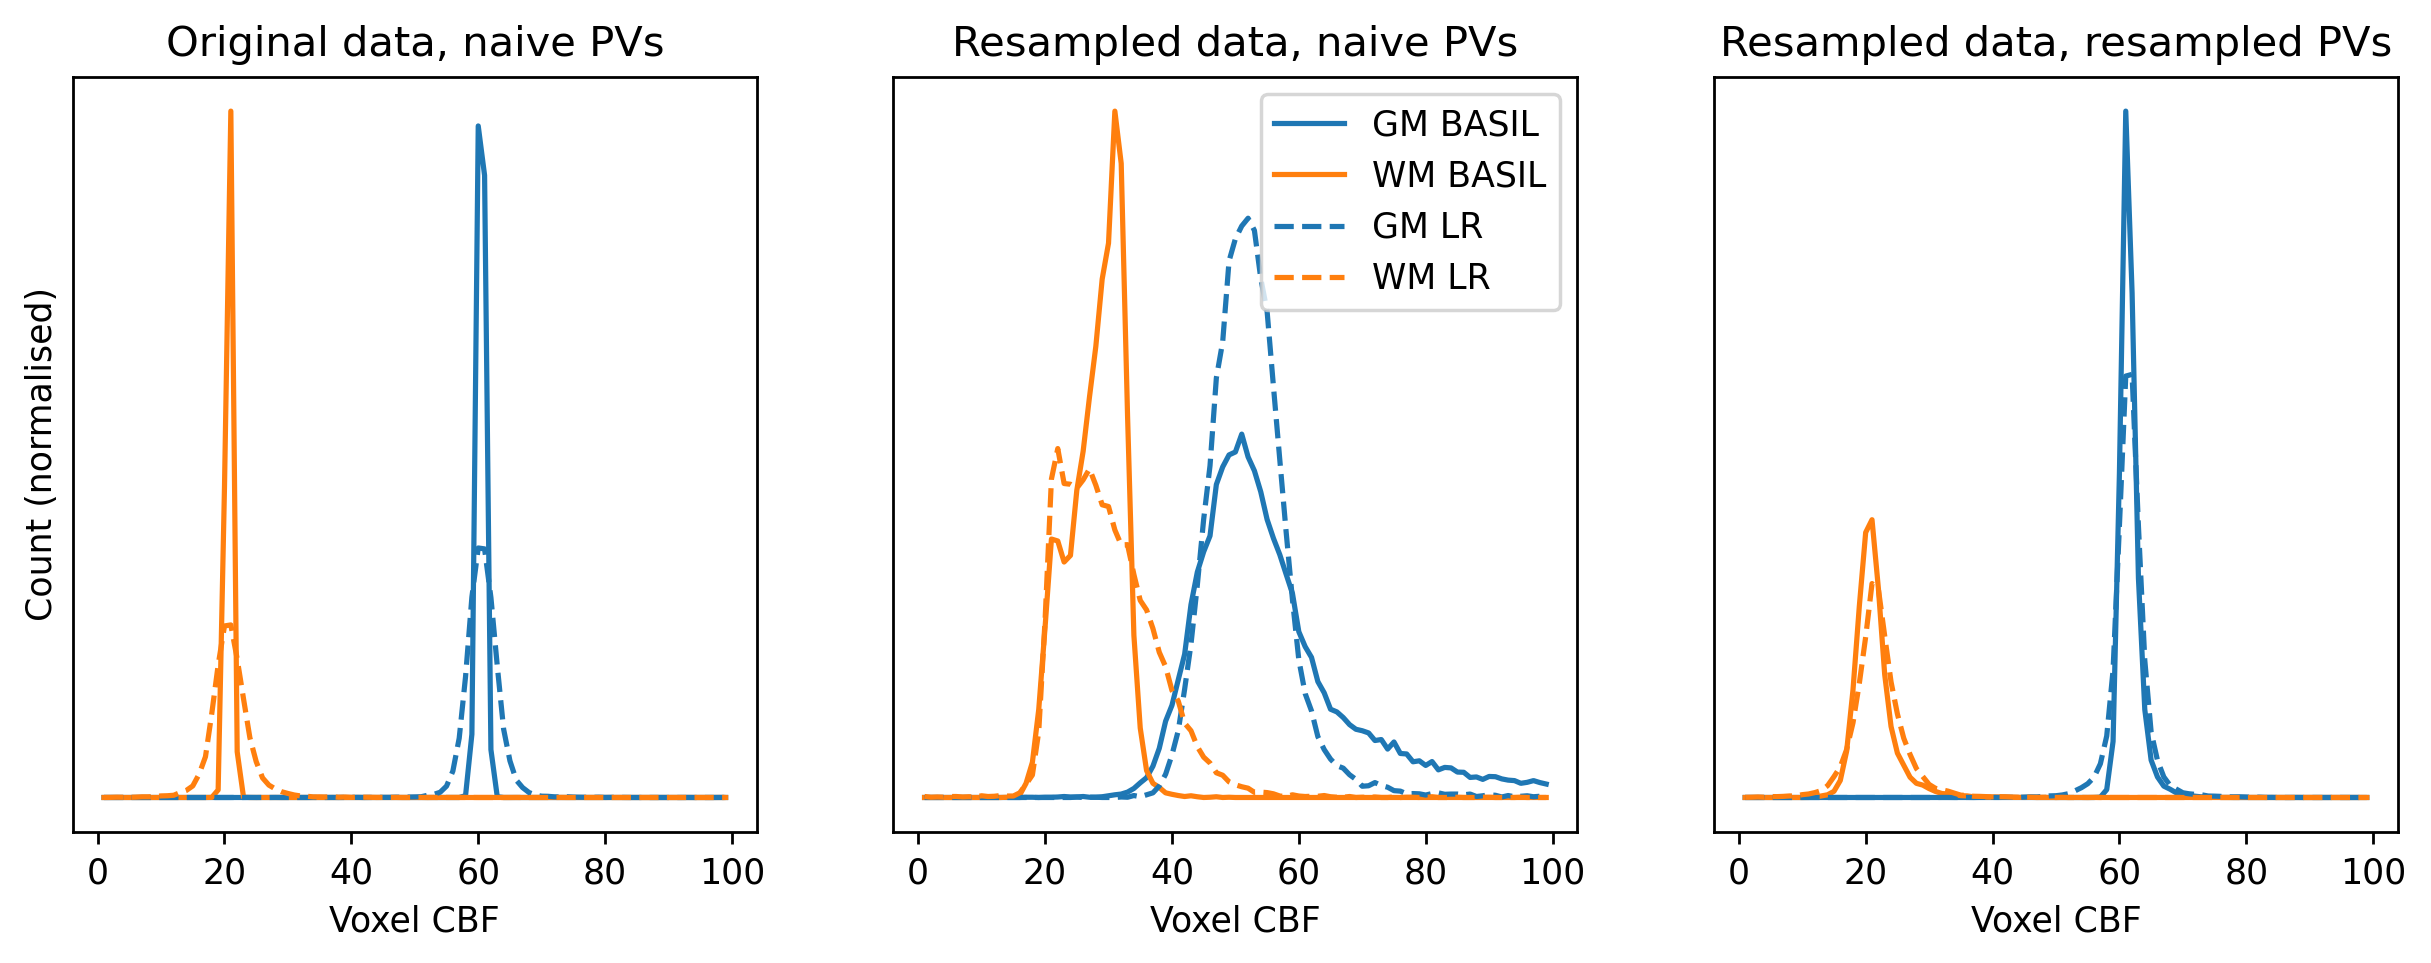
\includegraphics[width = \textwidth]{sim_asl_resamp_pvec.png}
\caption{Outcomes of PVEc on data before and after resampling. Left: for the base case of no resampling, PVEc of either form was able to recover ground truth CBF values for both tissues. Centre: after resampling, PVEc with the naive PV estimates led to poor recovery of ground truth. BASIL particularly struggled for GM whereas the LR method struggled for WM. Right: PVEc of the resampled data with the resampled PV estimates led to excellent recovery of ground truth, a result that was almost identical to the base case without resampling.}
\label{sim_asl_resamp_pvec}
\end{figure}

Figure \ref{sim_asl_resamp_pvec} shows the outcomes of PVEc on the high SNR simulation data before and after resampling. PVEc of either form on the original data was able to recover the ground truth values for GM and WM CBF. Following a round-trip of resampling, PVEc with the naive PV estimates led to poor recovery of ground truth for either method. BASIL displayed positive skew in GM but was more symmetric in WM, whereas the reverse was true for the LR method. Finally, PVEc with the double-resampled PV estimates showed a substantial improvement over the naive approach; the results were essentially identical to the base case established without resampling. 

\begin{figure}[H]
\centering
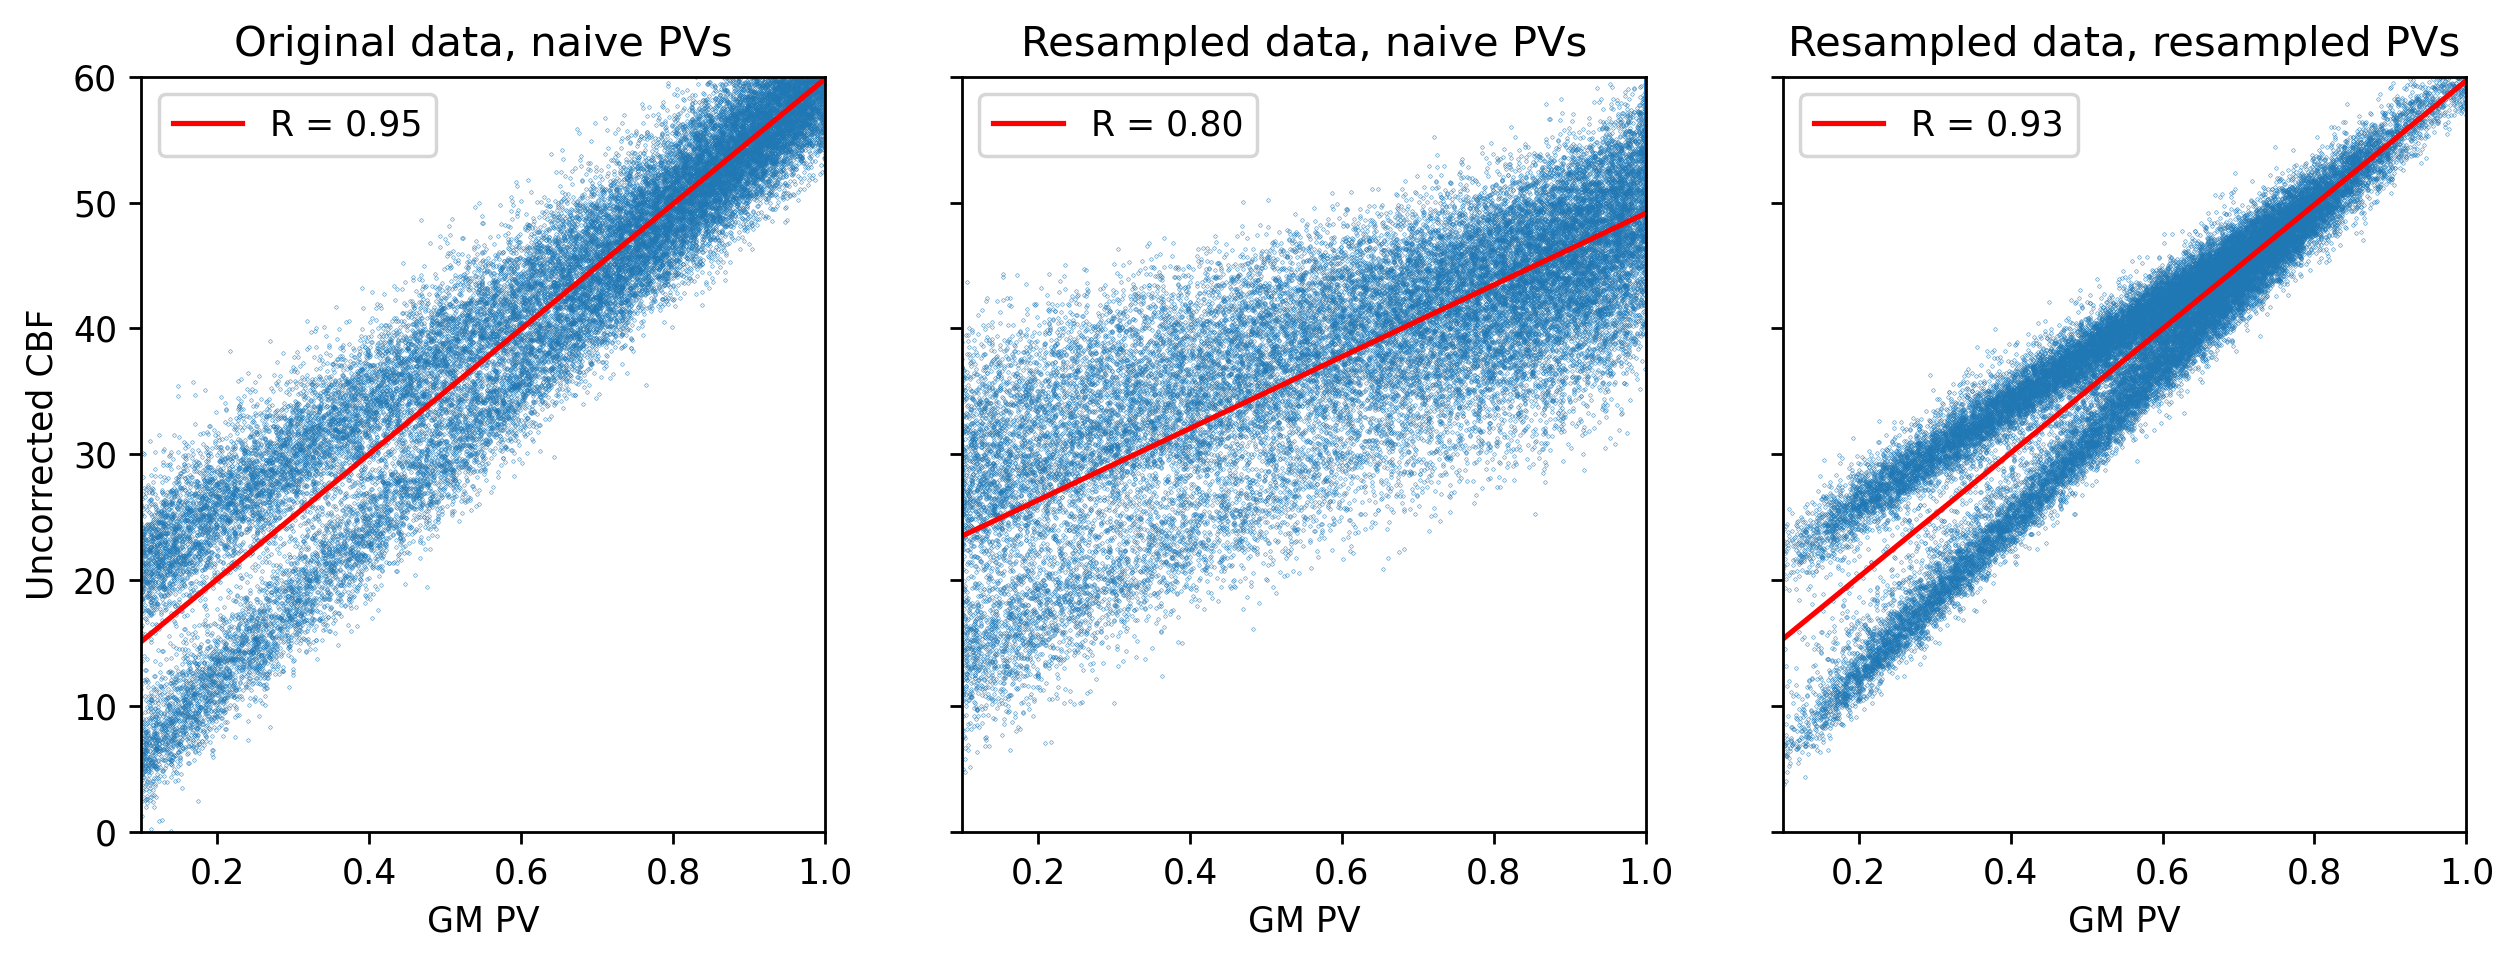
\includegraphics[width = \textwidth]{sim_asl_resamp_scatter.png}
\caption{Scatter plots of uncorrected CBF against GM PV before and after resampling. Left: the base case of no resampling showed a very strong correlation coefficient ($R$ = 0.95). Centre: a scatter of CBF from resampled data against naive GM PV showed a substantial decrease in $R$ to 0.79, indicating that the naive PVs did not correlate with the PVE of the data as well. Right: scatter against the resampled GM PV, which showed an increase in $R$ to 0.89. This indicated that the resampled PVs better reflect the PVE that were actually embedded in the data after resampling.}
\label{sim_asl_resamp_scatter}
\end{figure}

Figure \ref{sim_asl_resamp_scatter} shows voxelwise scatter plots of GM PV against uncorrected CBF derived from the high SNR simulation data before and after resampling. Linear regressions were performed in each case. Prior to resampling, there was an extremely strong relationship between CBF and GM PV with correlation coefficient ($R$ value) of 0.95. This reflects the nature in which the data was generated, namely in direct proportion to the PVs present in each voxel with no underlying parameter variation. The bimodal distribution of CBF could clearly be observed in the two separate lines that the voxels clustered around. Following resampling of the ASL data, a scatter of CBF against naive GM PV showed a substantial decrease in $R$ to 0.79. This decrease indicated that the naive PVs no longer explained the variance observed in the resampled data to the same extent as before. Finally, a scatter against the double-resampled GM PV showed an improvement in $R$ to 0.89, 
largely recovering the original value in the base case. The increase in $R$ value indicated that the double-resampled PVs better matched the extra PVE that were embedded within the data following resampling. 

\begin{figure}[H]
\centering
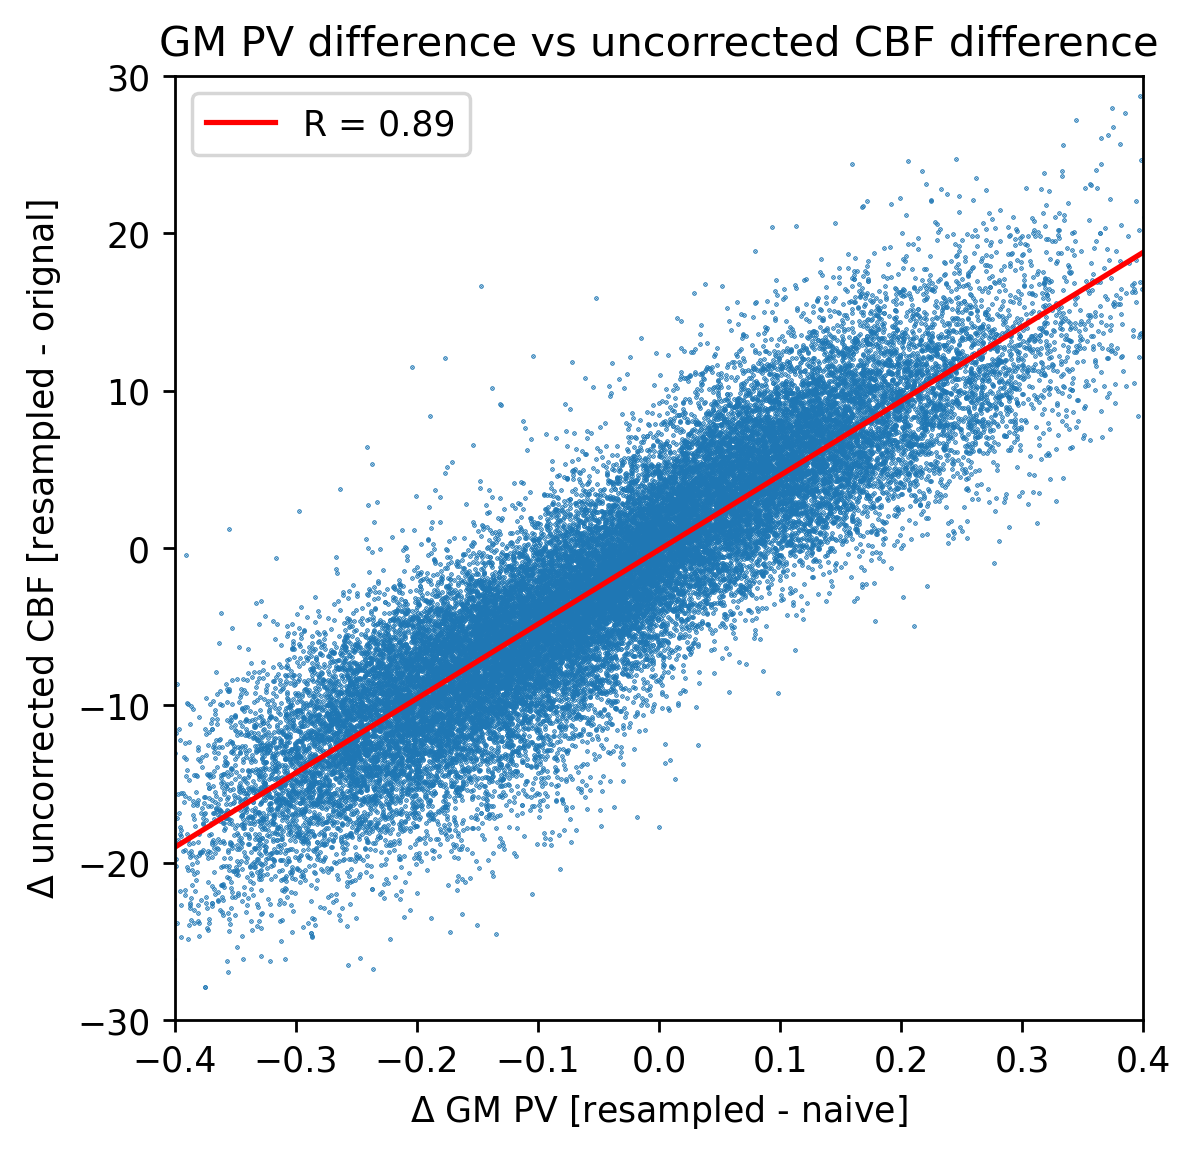
\includegraphics[width = 0.6\textwidth]{sim_asl_deltapv_deltacbf.png}
\caption{Scatter plot of change in GM PV against change in uncorrected CBF. Change in either quantity was defined as the resampled variable minus the original. The high correlation coefficient demonstrated that the change in CBF arising due to resampling of the ASL data could almost entirely be explained by a change in the corresponding voxel PV.}
\label{sim_asl_deltapv_deltacbf}
\end{figure}

Figure \ref{sim_asl_deltapv_deltacbf} shows a scatter plot of change in GM PV against change in uncorrected CBF before and after resampling. For both quantities, the change was defined as the resampled variable minus the original (for example, CBF of resampled data minus CBF of original). A high correlation coefficient was observed ($R$ = 0.89), which implied that the change in uncorrected CBF was largely explained by a corresponding change in GM PV. This shows that applying the same resampling to the PV estimates does convey meaningful information about the extra PVE that are introduced into the ASL data. For voxels that lost GM as a result of resampling, uncorrected CBF was reduced, which was in agreement with the theoretical foundations of PVE. 

\subsubsection{Low SNR repeats}

\begin{figure}[H]
\centering
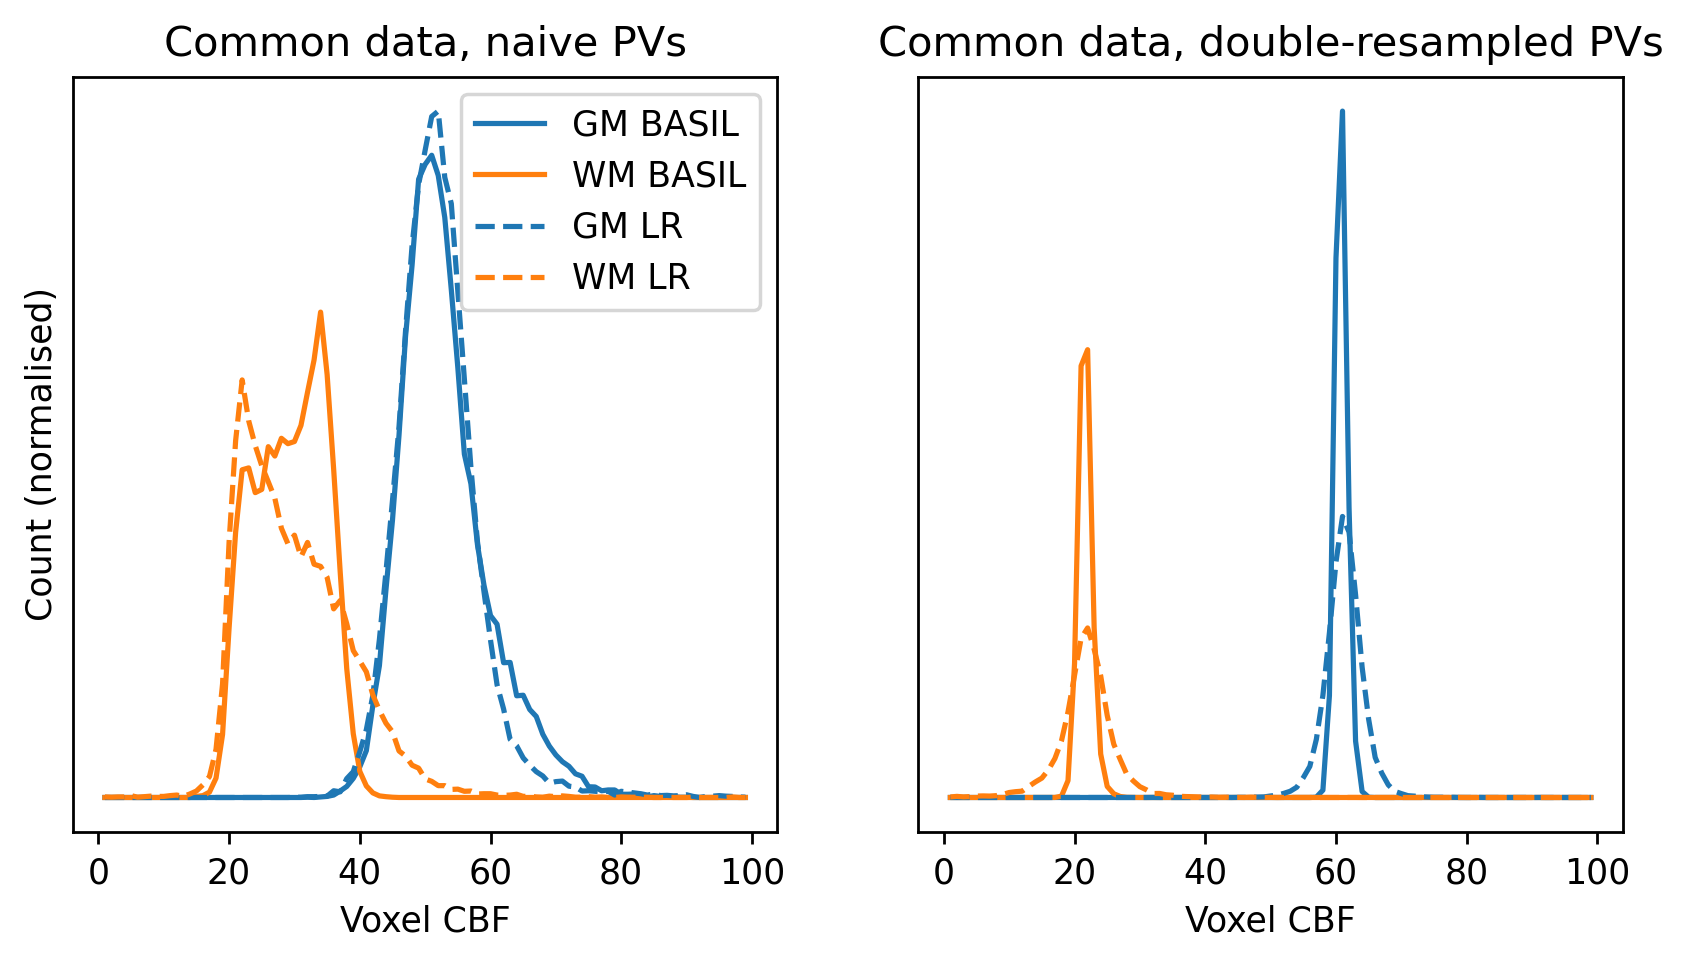
\includegraphics[width = 0.75\textwidth]{sim_rpts_resamp_pvec.png}
\caption{Histograms of PVEc CBF for simulated repeat data in common analysis space. The mean distribution across repeats is shown. Left: PVEc with the naive PV estimates led to a poor recovery of ground truth, whereas (Right:) PVEc with the double-resampled PV estimates performed much better. Both of these findings were in agreement with the results of the high SNR simulation shown in figure \ref{sim_asl_resamp_pvec}.}
\label{sim_rpts_resamp_pvec}
\end{figure}

Figure \ref{sim_rpts_resamp_pvec} shows histograms of PVEc CBF on the simulated repeat data in common analysis space. In both plots the mean distribution across repeats is shown. PVEc of the common-aligned data with naive PVs showed poor recovery of the ground truth, whereas PVEc with double-resampled PVs showed a significant improvement in recovery of the ground truth distributions. Both of these results were in agreement with those observed on the high SNR simulation (figure \ref{sim_asl_resamp_pvec}). This result implied that accurately conveying the different PVE embedded within repeat data is key to successful PVEc in a non-native analysis space.  

\begin{figure}[H]
\centering
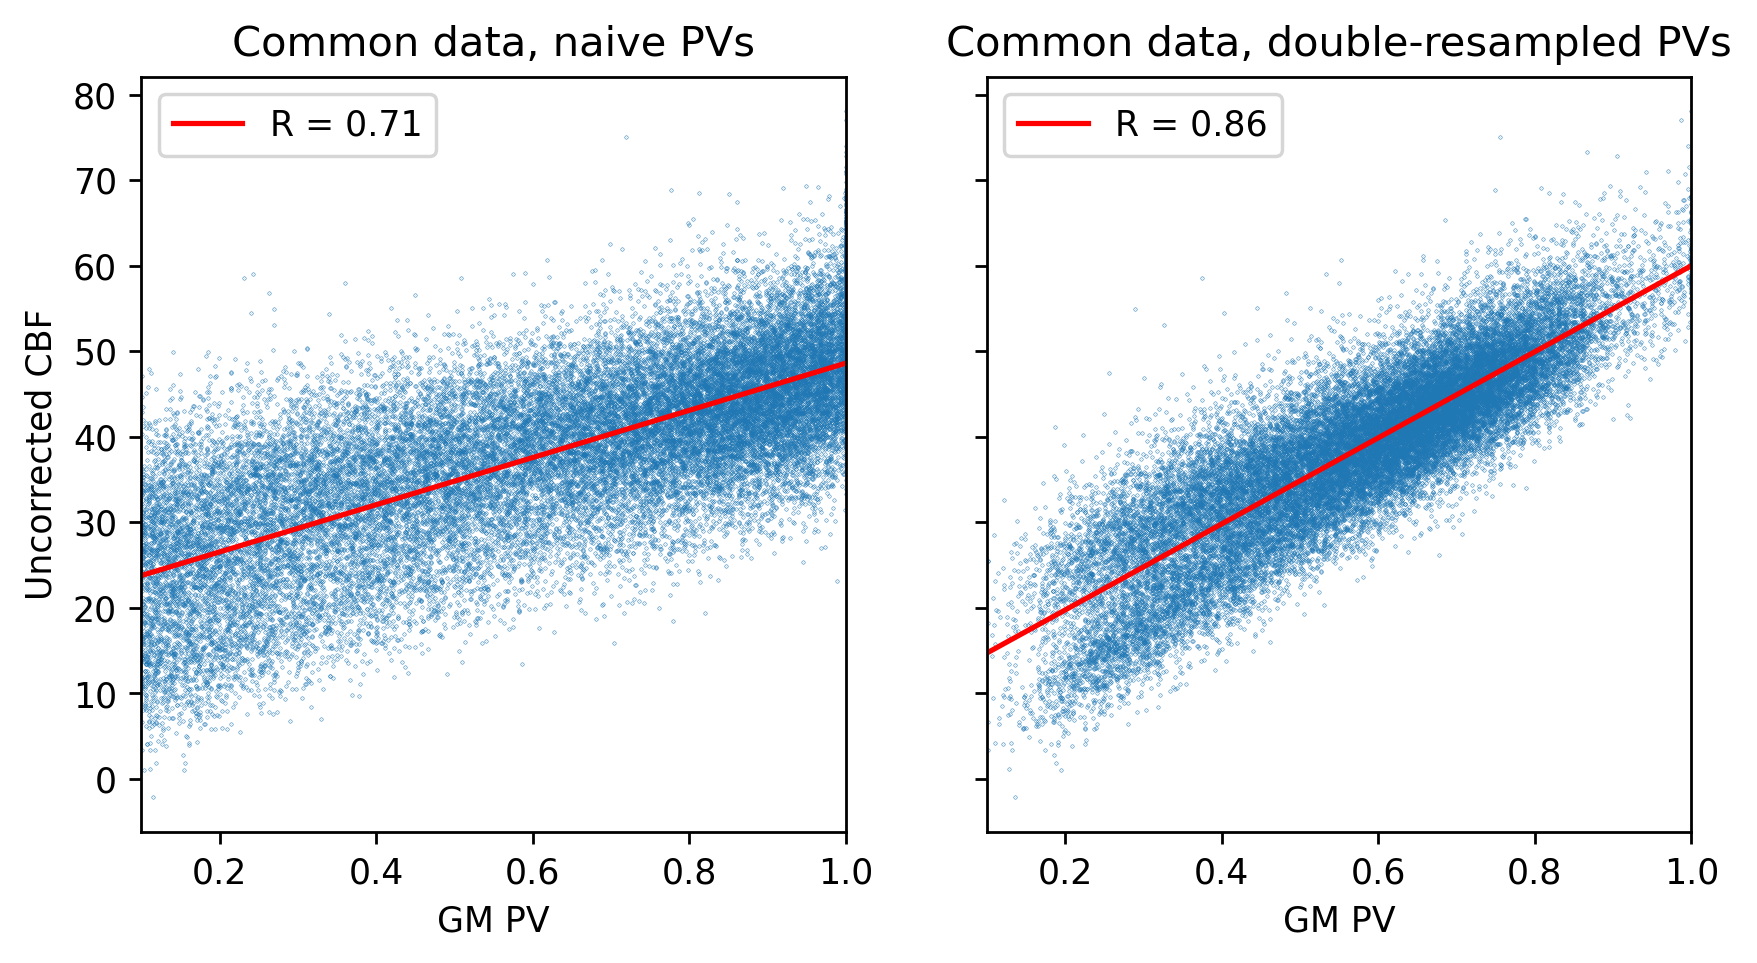
\includegraphics[width = 0.75\textwidth]{sim_rpts_resamp_scatter.png}
\caption{Scatter plots and linear regressions of uncorrected CBF for a single repeat of simulated data in common space. Left: a scatter against naive GM PV; Right: a scatter against double-resampled GM PV. The correlation coefficient for the double-resampled PVs was stronger, indicating that they better explained the variability seen in the data.}
\label{sim_rpts_resamp_scatter}
\end{figure}

Figure \ref{sim_rpts_resamp_scatter} shows scatter plots and linear regressions of uncorrected CBF estimated from the repeat data in common analysis space. The regressions were performed against the naive GM PV estimates and the double-resampled GM PV estimates (a single repeat's worth of data was used). Again mirroring the results from the high SNR simulation case (figure \ref{sim_asl_resamp_scatter}), the correlation coefficient for the double-resampled PVs was greater than for the naive PVs ($R$ = 0.81 vs. 0.71). This showed that the double-resampled PVs better matched the PVE that were embedded within the ASL data after resampling into the common space. Both correlation coefficients were smaller than the high SNR case, which was presumed to be due to the presence of increased noise in the repeat data. 


\begin{figure}[H]
\centering
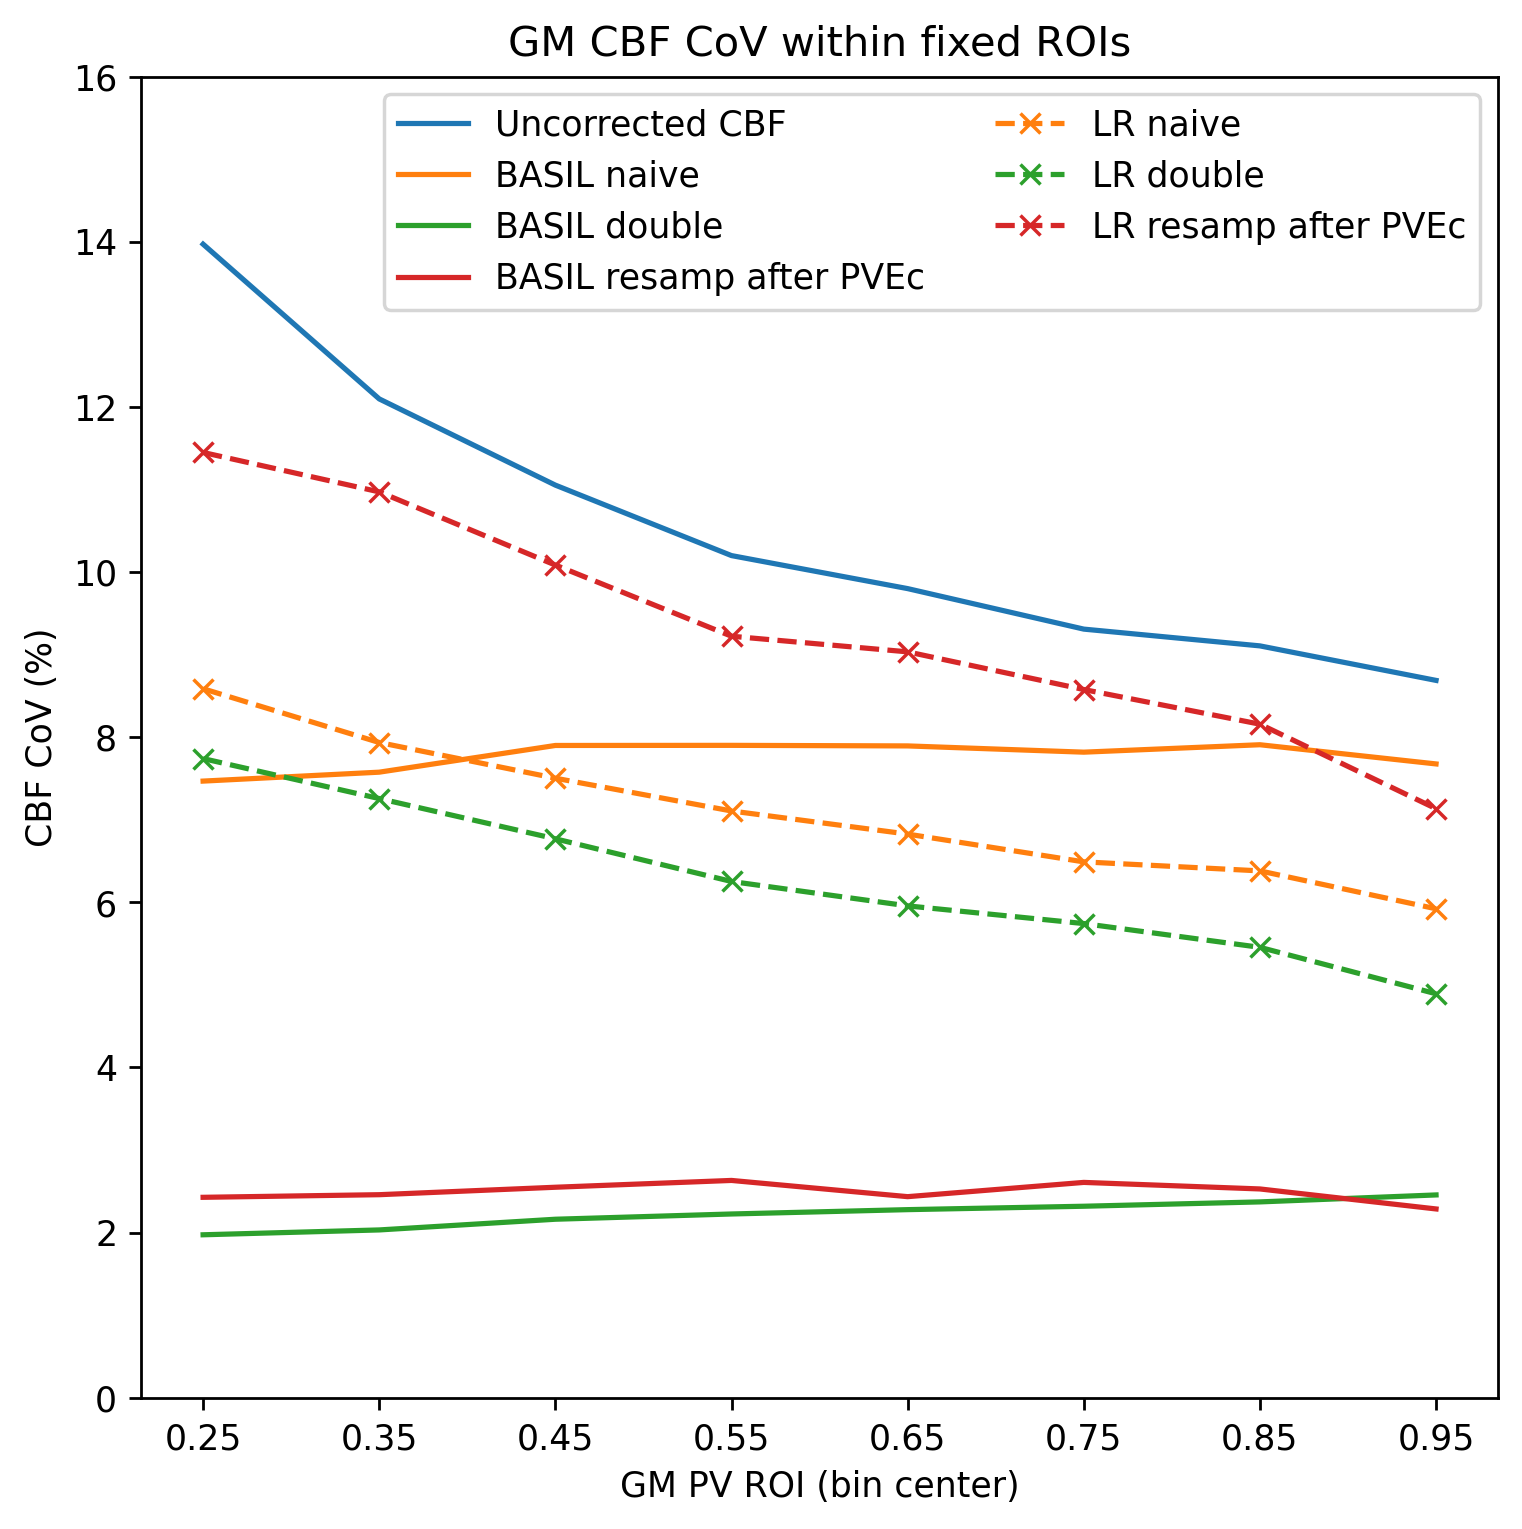
\includegraphics[width = 0.6\textwidth]{sim_lowsnr_cov.png}
\caption{CoV of CBF measurement in common analysis space across simulated repeats. The blue trace represents the baseline case of no PVEc. For both BASIL and the LR method, PVEc with double-resampled PV estimates (green) resulted in smaller CoV than for naive PV estimates (orange).}
\label{sim_lowsnr_cov}
\end{figure}

Figure \ref{sim_lowsnr_cov} shows the coefficient of variation across all simulated repeats for CBF measurement within voxel ROIs. The baseline case of uncorrected CBF was established: this was expected to lead to a higher CoV, due to the differing levels of PVE within the individual repeats feeding through to their resultant CBF estimates. CoV of uncorrected CBF decreased for ROIs defined with a higher proportion of GM PV, which was in agreement with theory (in the limit, voxels that are pure GM should have identical CBF due to the assumption of constant CBF underpinning these simulations). For both BASIL and the LR method, PVEc with double-resampled PV estimates resulted in lower CoV than with the naive PV estimates. BASIL's double-resampled PVEc led to the lowest CoV for all ROIs of all methods, whereas BASIL's naive PVEc actually returned higher CoV than the baseline case of uncorrected CBF. 

\subsection{\textit{In-vivo} data}

\subsubsection{High SNR data}

\begin{figure}[H]
\centering
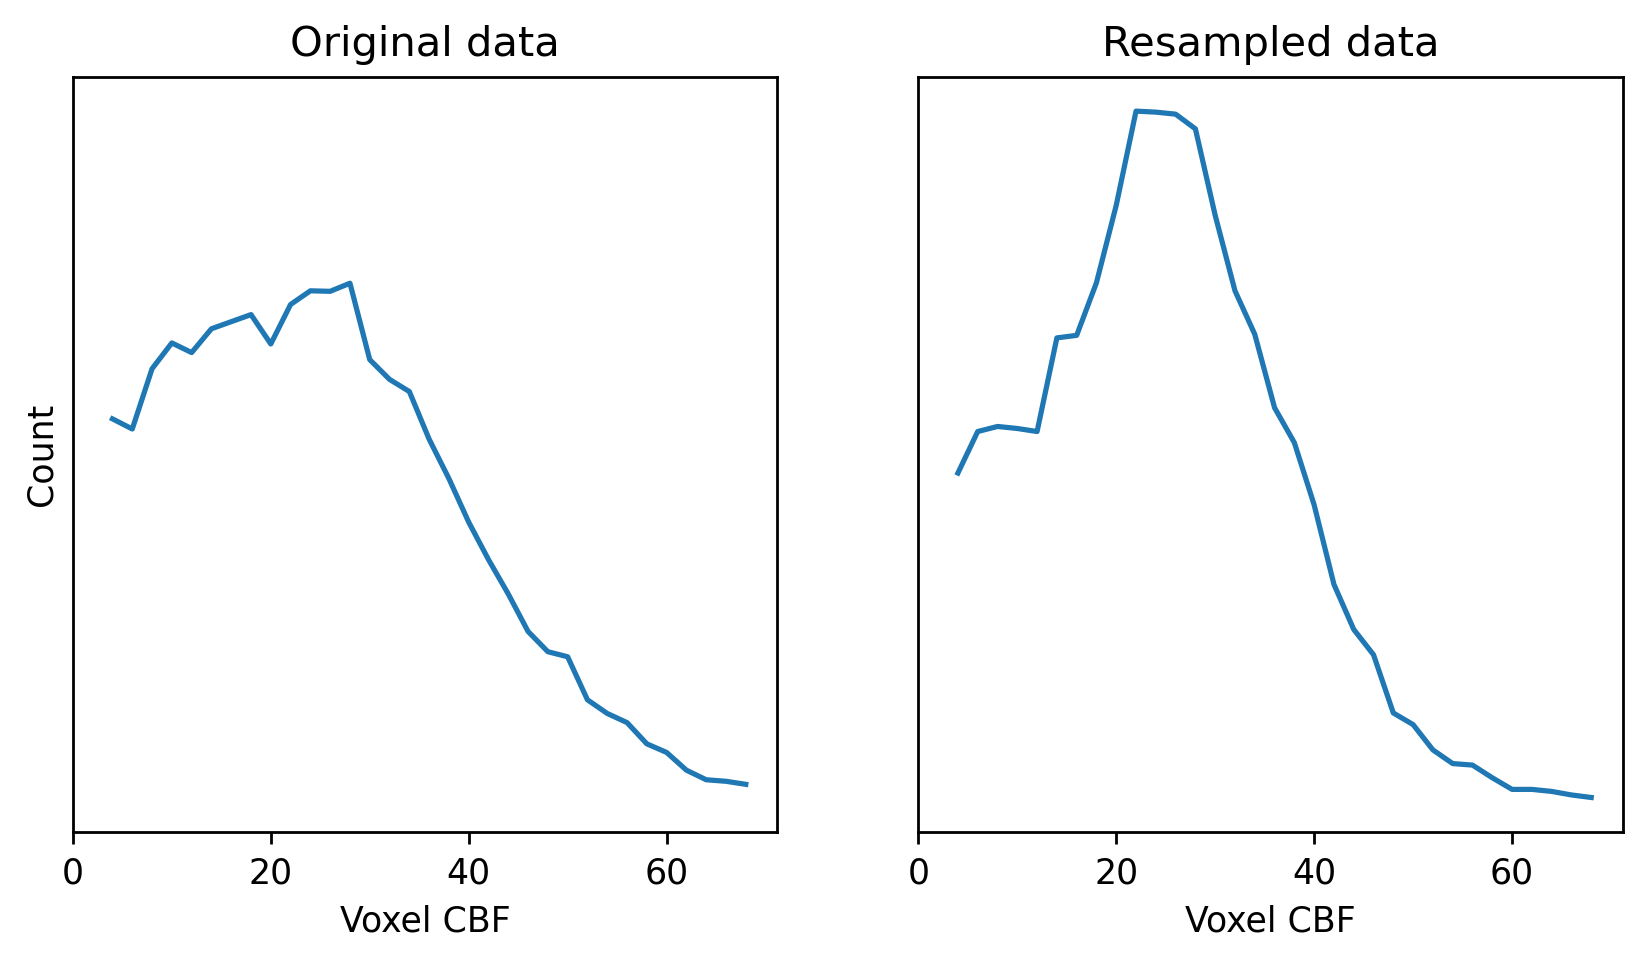
\includegraphics[width = 0.75\textwidth]{real_resamp_hist.png}
\caption{Distributions of uncorrected CBF from the high SNR \textit{in-vivo} data before (left) and after (right) resampling. The effect of resampling was to shift the peak of the distribution from around 0 units to 10, making it more Gaussian and consistent with increasing PVE within the data.}
\label{real_resamp_hist}
\end{figure}

Figure \ref{real_resamp_hist} shows uncorrected CBF estimated from the high SNR \textit{in-vivo} data, before and after a round-trip of resampling. The distribution was not bimodal (as was the case for the high SNR simulation case in figure \ref{sim_asl_resamp_hist}); instead it was monotonic decreasing for increasing CBF. After a round-trip of resampling, the the peak of the distribution shifted substantially (from around 0 units to 10 units). Though the exact nature of the distribution was somewhat different to the idealised case established in the simulations, the effect of resampling was nevertheless to substantially alter the distribution and make it look more Gaussian, consistent with increasing PVE.  
 
\begin{figure}[H]
\centering
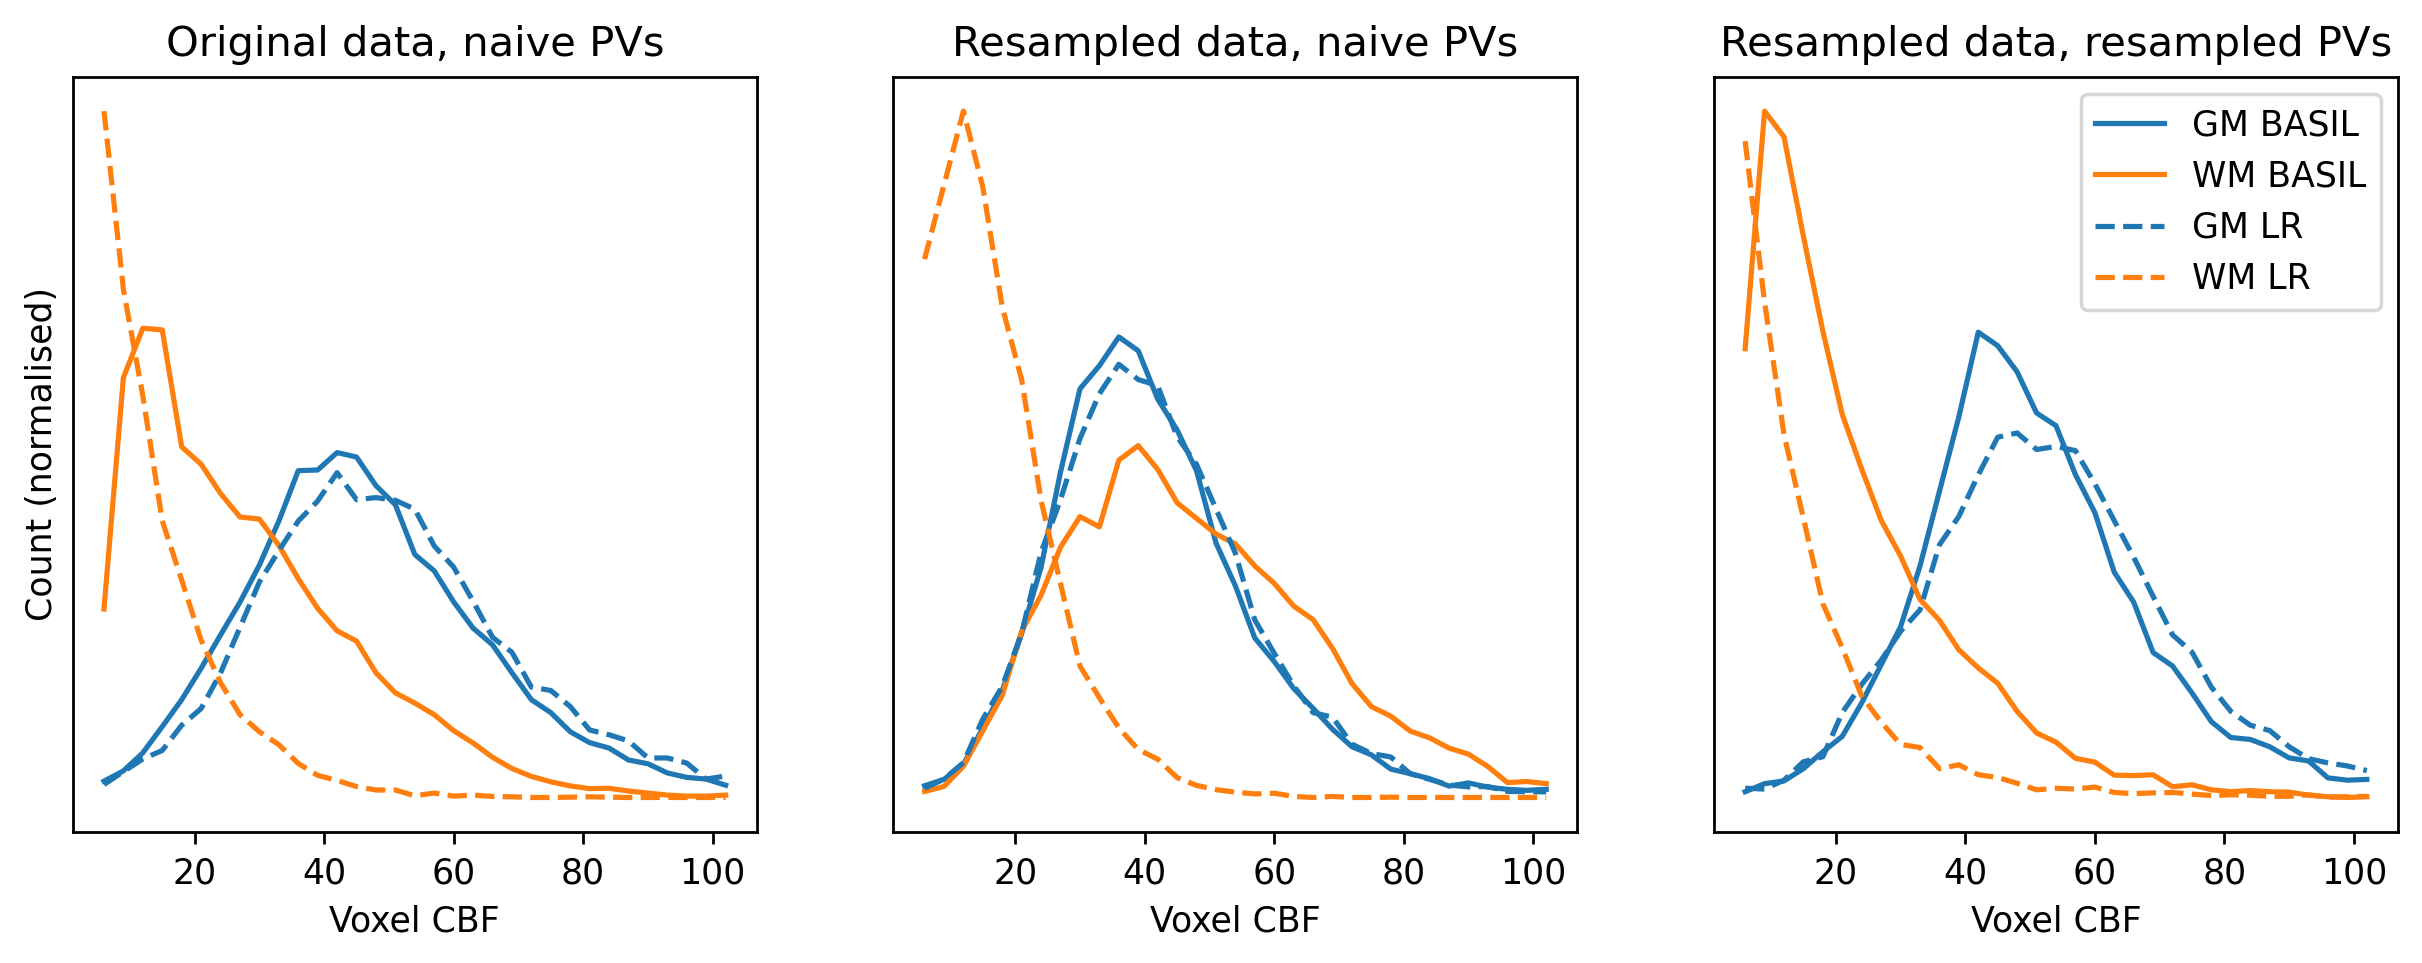
\includegraphics[width = \textwidth]{real_resamp_pvec.png}
\caption{Outcomes of PVEc before and after resampling. Left: original data with naive estimates; Centre: resampled data with naive estimates; Right: resampled data with resampled estimates. The former case (left) was taken to establish the baseline result; PVEc of resampled data with resampled PVs (right) led to a more similar result than with the naive estimates (centre).}
\label{real_resamp_pvec}
\end{figure}

Figure \ref{real_resamp_pvec} shows the outcomes of PVEc on the high SNR \textit{in-vivo} data before and after resampling. PVEc of the original data with the naive PVs established the expected distributions in the baseline case. PVEc of resampled data with naive PVs led to different distributions, particularly for BASIL's WM result which showed a positive skew. Both BASIL and the LR method returned a similar distribution for GM. PVEc of resampled data with resampled PVs resulted in distributions that more closely matched the baseline case (particularly for BASIL's WM result). These two findings (firstly, the choice of naive or resampled PVs affected the outcome of PVEc, and secondly, PVEc of resampled data with resampled PVs better matched the baseline case in native space), both matched the corresponding simulation results shown in figure \ref{sim_asl_resamp_pvec}. 


\begin{figure}[H]
\centering
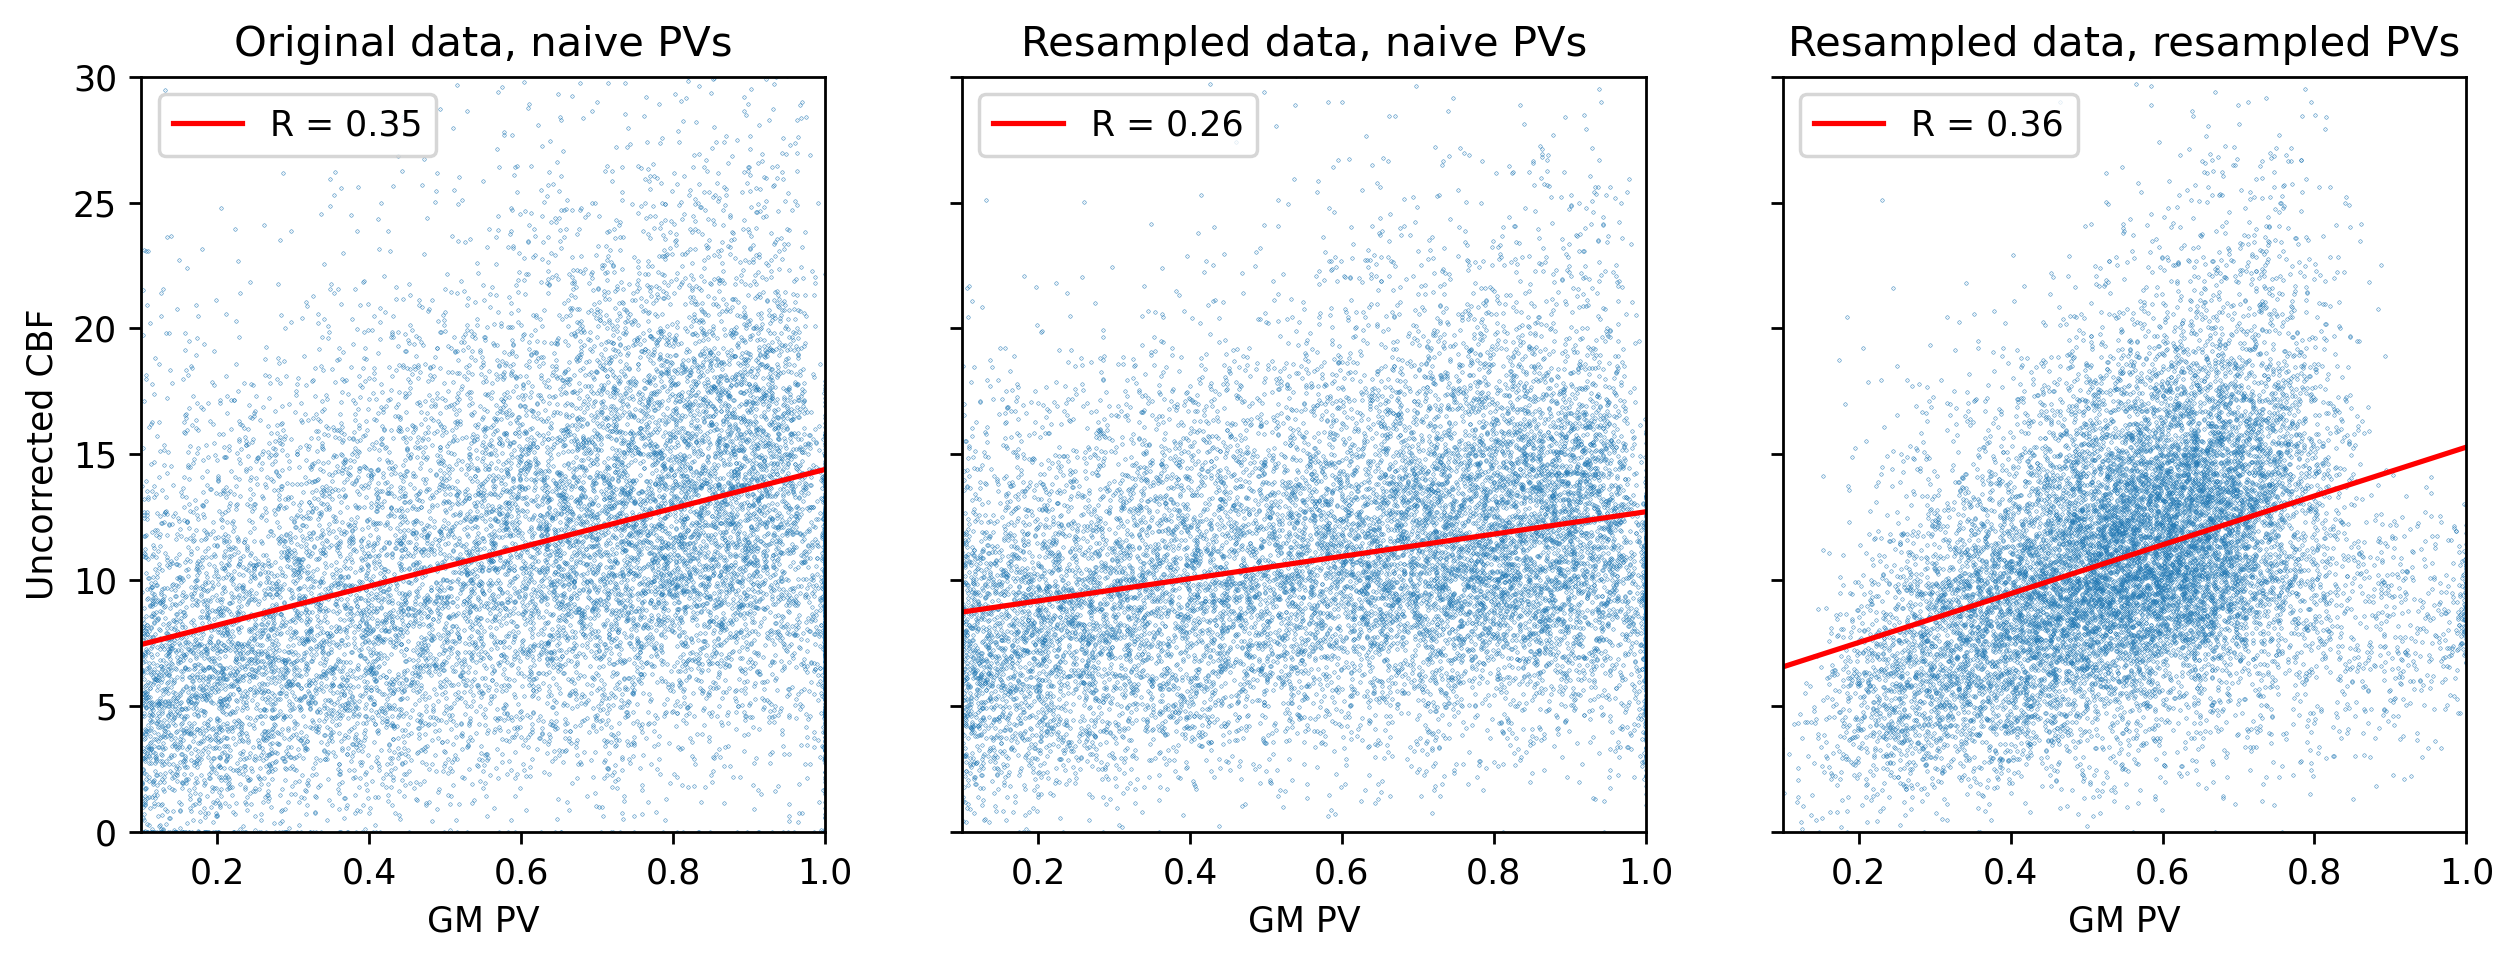
\includegraphics[width = \textwidth]{real_highsnr_scatter.png}
\caption{Scatter plots and linear regressions of uncorrected CBF estimated from data before and after resampling. Left: a scatter of the original data against the naive GM PV estimates established the baseline case, correlation coefficient $R$ = 0.35. Centre: a scatter of resampled data against the naive GM PVs resulted in a reduction of $R$ to 0.26. Right: a scatter of resampled data against resampled PVs showed an increase in $R$ to 0.36, matching the baseline case.}
\label{real_highsnr_scatter}
\end{figure}

Figure \ref{real_highsnr_scatter} shows scatter plots and linear regressions of uncorrected CBF for the high SNR \textit{in-vivo} data before and after resampling. The regression of original data against the naive PVs established the baseline case with a correlation coefficient $R$ of 0.35. Regression of the resampled data against the naive PVs resulted in an $R$ value of 0.26, whereas regression of the resampled data against the resampled PVs resulted in an $R$ of 0.36. This indicated that the double-resampled PVs better matched the PVE that were embedded within the resampled ASL data, a finding in agreement with the simulations shown in figure \ref{sim_asl_resamp_scatter}. 

\begin{figure}[H]
\centering
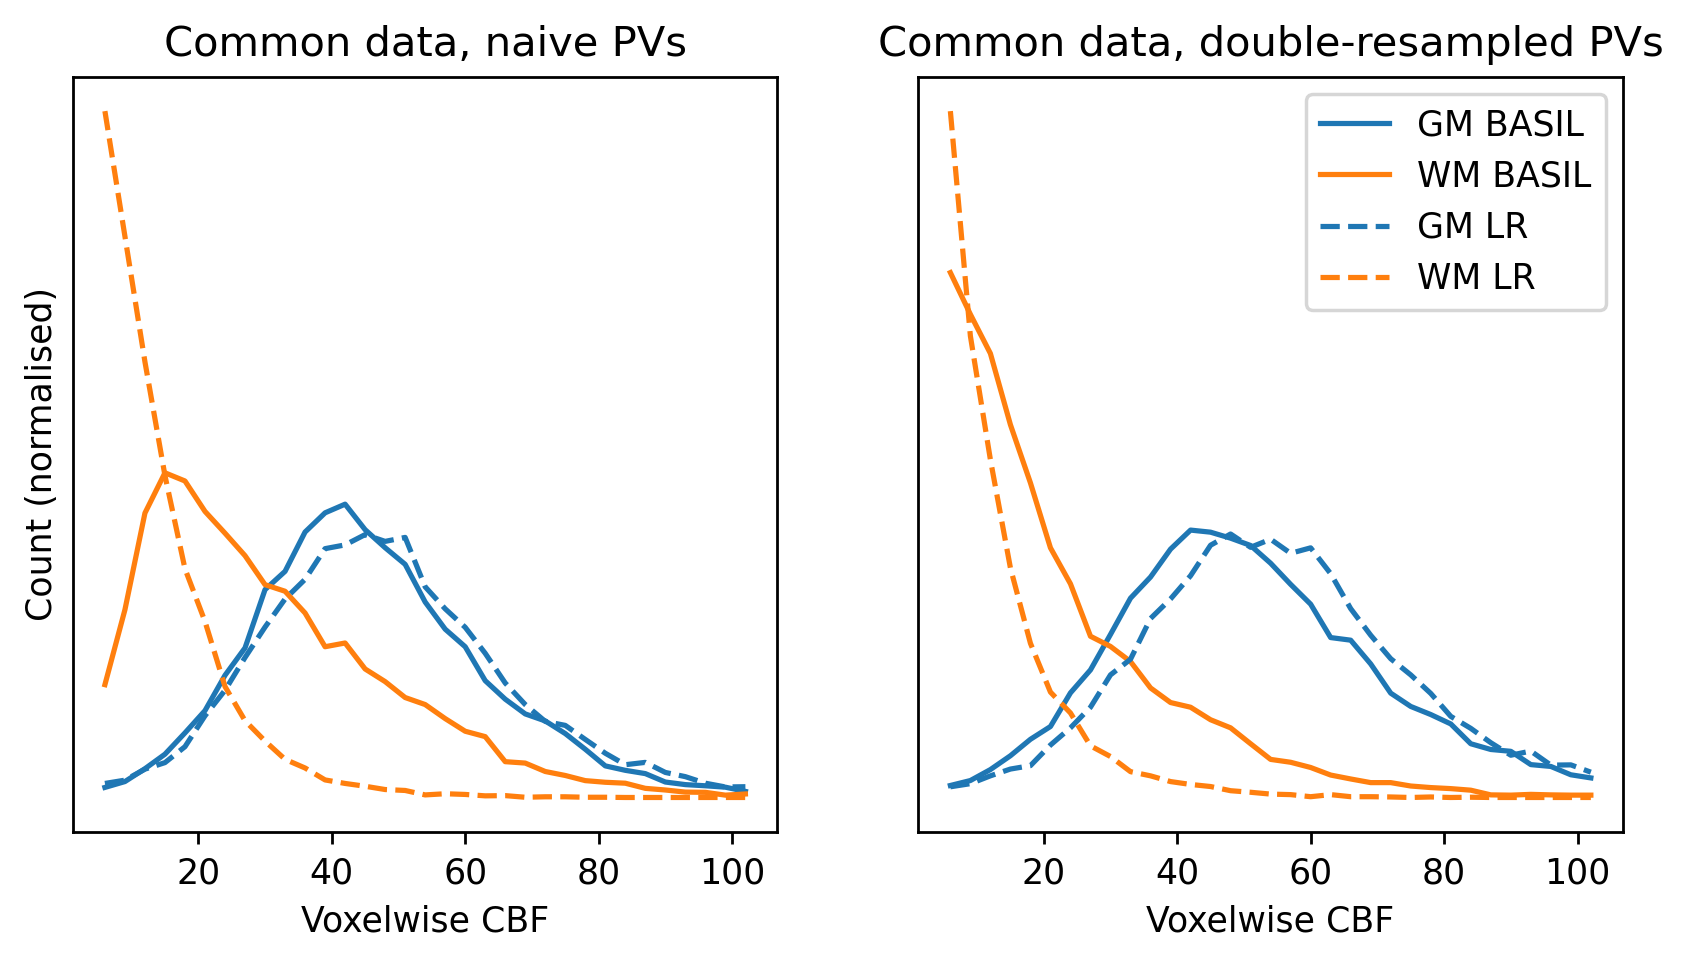
\includegraphics[width = 0.75\textwidth]{real_highsnr_pvec_cmn.png}
\caption{Outcomes of PVEc in common space, high SNR \textit{in-vivo} data. Left: PVEc with naive PV estimates. Right: PVEc with double-resampled PV estimates. Distributions of GM CBF were similar in either case. BASIL's WM distribution did alter noticeably;  double-resampled PVs led to better separation of tissue CBF compared to the naive case.}
\label{real_highsnr_pvec_cmn}
\end{figure}

Figure \ref{real_highsnr_pvec_cmn} shows the outcome of PVEc on the high SNR \textit{in-vivo} data after resampling into a common structural-aligned space. It is difficult to establish a baseline case in this situation because the ASL data has necessarily been resampled into a common space for analysis, thereby increasing the extent of PVE in the data in an unpredictable manner. BASIL's PVEc of the common aligned data with the naive PVs resulted in different distributions of GM and WM CBF than PVEc with the double-resampled PVs. In particular, PVEc with the double-resampled PVs resulted in better separation of the GM and WM CBF distributions for BASIL, a finding that matched the trends seen in acquisition-native space (figure \ref{real_resamp_pvec}).

\begin{figure}[H]
\centering
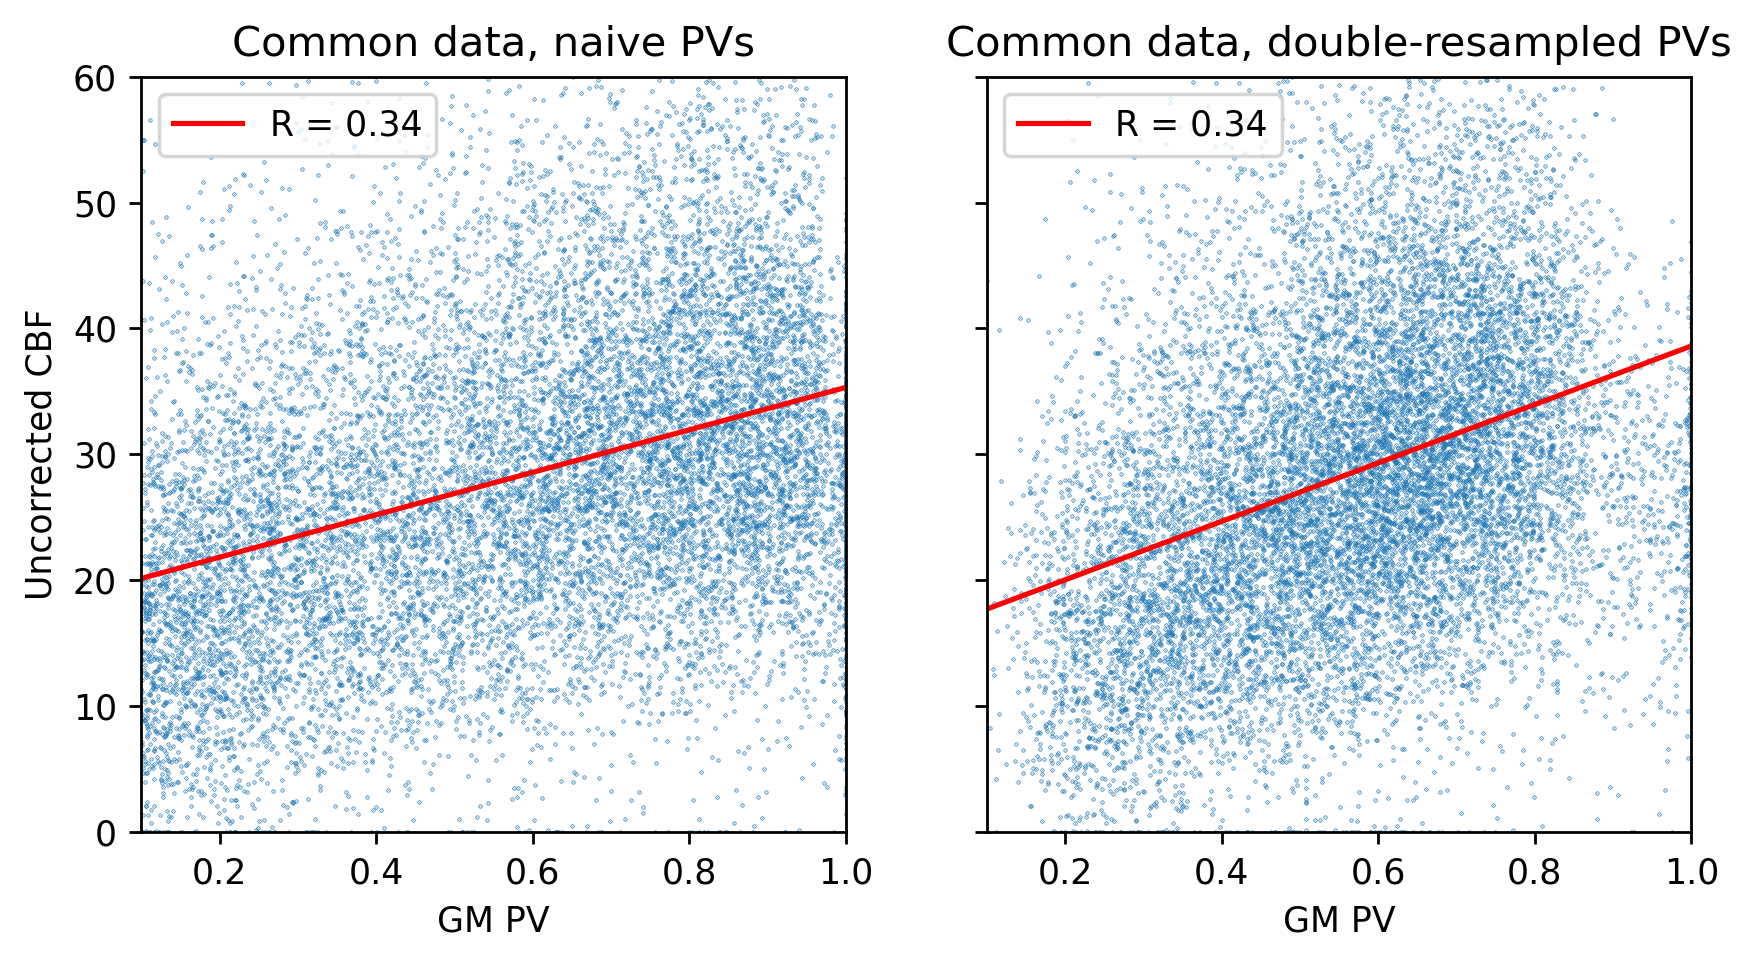
\includegraphics[width = 0.75\textwidth]{real_highsnr_scatter_cmn.png}
\caption{Scatter plots and linear regressions of uncorrected CBF in a common analysis space for the high SNR \textit{in-vivo} data. Left: regression against naive GM PV estimates. Right: regression against double-resampled GM PV estimates, with a slightly higher correlation coefficient (0.37 instead of 0.35).}
\label{real_highsnr_scatter_cmn}
\end{figure}

Figure \ref{real_highsnr_scatter_cmn} shows scatter plots and linear regressions of uncorrected CBF in a common analysis space estimated from the high SNR \textit{in-vivo} data. When regressed against the double-resampled GM PV estimates, there was a marginally higher correlation coefficient ($R$ = 0.37 instead of 0.35 with naive estimates). 

%
%\begin{figure}[H]
%\centering
%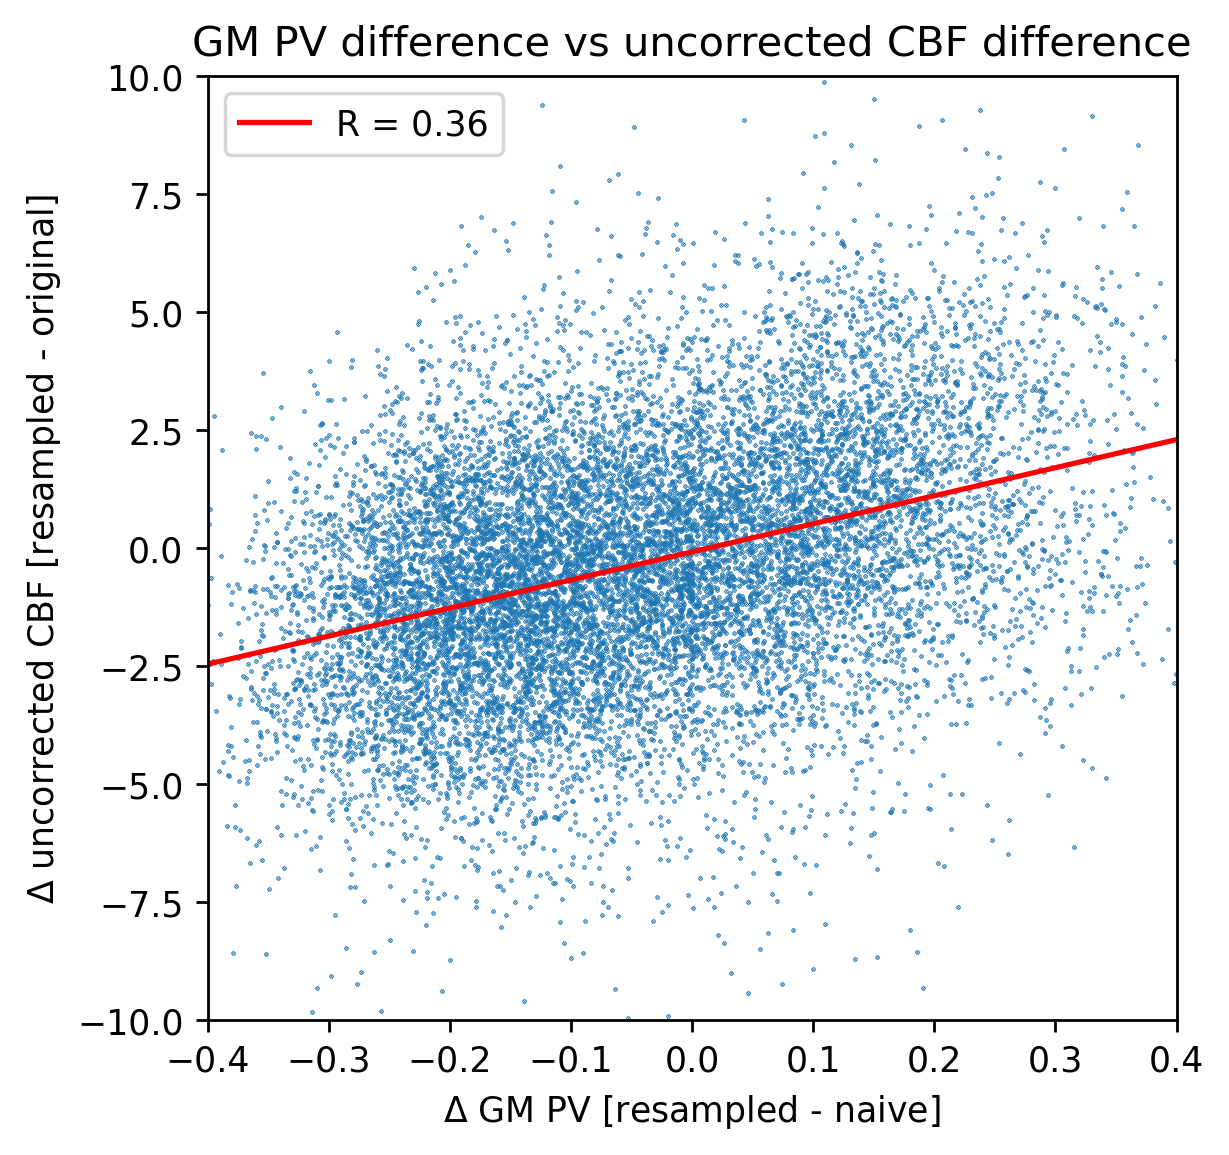
\includegraphics[width = 0.5\textwidth]{real_highsnr_deltagm_deltacbf.png}
%\caption{}
%\label{real_highsnr_deltagm_deltacbf}
%\end{figure}


\subsubsection{Low SNR repeats}


\begin{figure}[H]
\centering
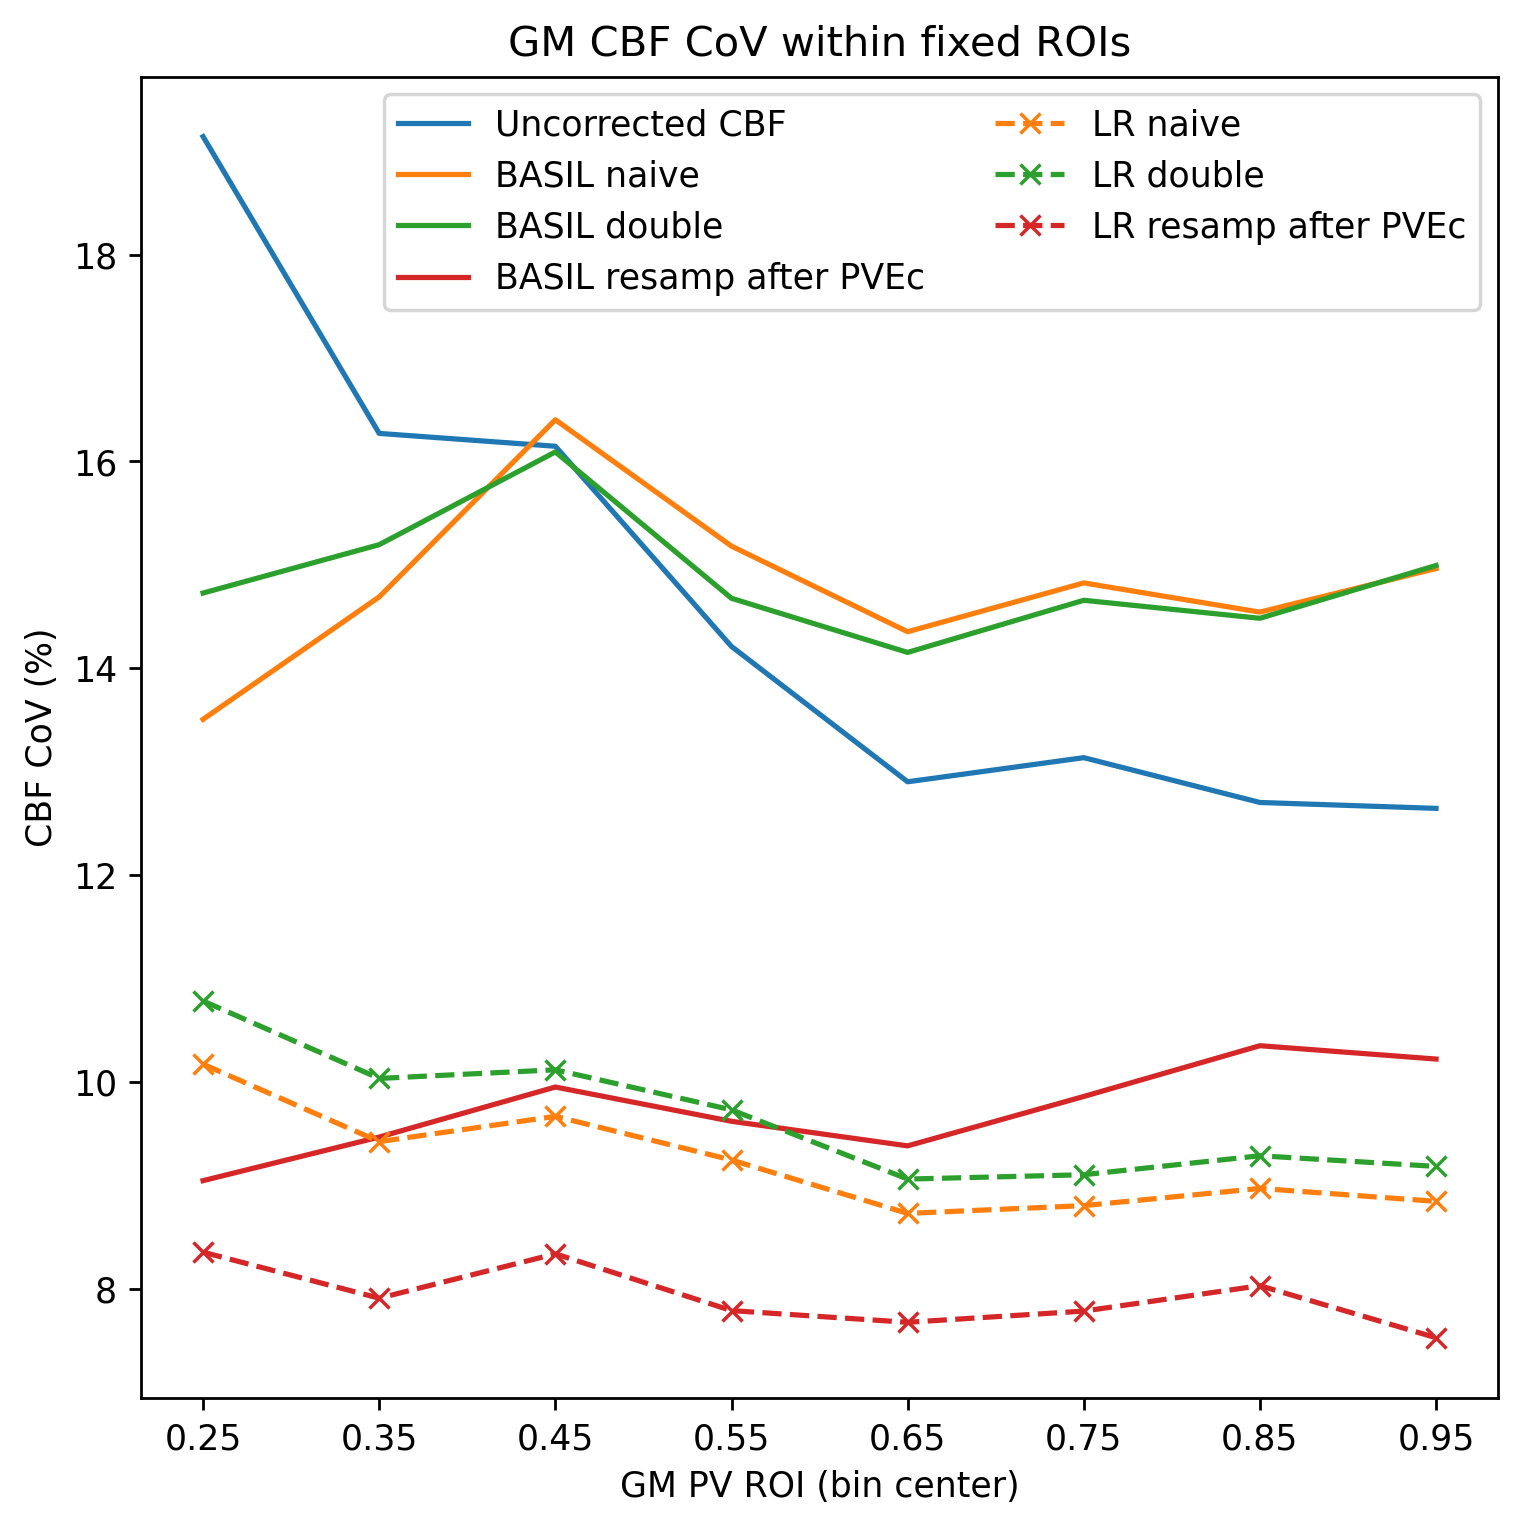
\includegraphics[width = 0.6\textwidth]{real_lowsnr_cov.png}
\caption{CoV in CBF measurement across the \textit{in-vivo} repeat data in common space. The trace of uncorrected CBF established the baseline case; CoV decreased with increasing GM PV. In general, LR methods returned substantially lower CoV than other methods, with the exception of BASIL resample after PVEc. The difference between naive (orange) and double-resampled (green) PVs was marginal for both the LR and BASIL methods. Resampling after PVEc gave the best performance for both PVEc methods.}
\label{real_lowsnr_cov}
\end{figure}

Figure \ref{real_lowsnr_cov} shows the CoV in CBF measurement across the \textit{in-vivo} repeat data in structural-aligned common space. The baseline case of uncorrected CBF was established; CoV decreased with increasing GM PV, in agreement with the simulated repeats (figure \ref{sim_lowsnr_cov}). All variants of the LR method returned substantially lower CoV than all variants of BASIL, with the exception of BASIL resample after PVEc, which returned broadly similar results. For both the LR method and BASIL, the difference between correction with naive PV estimates or double-resampled estimates was marginal. Within each PVEc method, the strategy of resampling after PVEc led to the lowest CoV values. 

\section{Discussion}

It is well known that resampling has the effect of smoothing data. This also increases the extent of PVE, which was readily observed in distributions of uncorrected CBF (figures \ref{sim_asl_resamp_hist} and \ref{real_resamp_hist}). The smoothing imposed by resampling also had a small noise-reducing effect which could be observed on the simulation experiments. Referring to the scatter plots in figure \ref{sim_asl_resamp_scatter}, the bimodal distribution of the original data resulted in two distinct linear clusterings, and the amount of noise was reflected in the spread of points around these clusterings. Following resampling, a bimodal distribution was again observed, but the spread of points around the clusterings was reduced, indicative of reduced noise within the data. 

If PVE are known to be present in the data, the results presented here imply native-space parameter estimation is preferable so as to avoid resampling which further increases PVE. There may of course be other justifications for analysing data in a non-native space that outweigh the importance of PVE. In such a situation, results from the simulations showed that PVEc with the double-resampling strategy was more successful than using naive PV estimates (figure \ref{sim_rpts_resamp_pvec}), but this result relied on the wholly unrealistic assumption of constant CBF in each tissue. For \textit{in-vivo} data, the difference between the naive and double-resampled strategies was more marginal, but the latter strategy nevertheless led to better separation of GM and WM CBF distributions (figure \ref{real_highsnr_pvec_cmn}) and a higher correlation coefficient of GM PV with uncorrected CBF (figure \ref{real_highsnr_scatter_cmn}). As such, it is concluded that obtaining PV estimates via double-resampling represents the best strategy for PVEc in non-native data space, but is nevertheless a compromise compared to native space parameter estimation. 

The reasoning behind the success of the double-resampled strategy is that it redistributes PVs between voxels in the same manner as signal is redistributed within the data that is being resampled. In this regard, one can draw a parallel with the emphasis placed on PSF-related effects in the PET PVE literature: resampling increases the effective PSF of data such that mixing of signal between voxels becomes problematic. Ironically, the importance of this result may actually increase as voxel size decreases, up to a point. Considering the example of a simple translation, for a fixed displacement of 1mm the amount of smoothing introduced when applied to a 2mm voxel grid would be greater than for a 4mm voxel grid (due to subvoxel effects, as illustrated in figure \ref{resamp_demo}). Hence, the resampling necessitated by a given transformation is more detrimental when applied to high resolution data than for low resolution. An alternative formulation is that data with low PVE stands to lose more information than data that contains high PVE; if one goes through the effort of obtaining data with low PVE, then one should strive to preserve that as much as possible during processing. 

In general, the results drawn from the \textit{in-vivo} data are harder to interpret because it is not known ahead of time what the `correct' result would look like. For example, the simulations used an assumption of constant CBF in both tissues so as to ensure any variance in CBF measurement could be explained by PVE. This clearly does not hold true for \textit{in-vivo} data. This likely explains, along with greater noise, why correlation coefficients of GM PV against uncorrected CBF (figure \ref{real_highsnr_scatter}) were lower across the board than for the simulation experiments. As for the repeatability of CBF measurement in repeat data, a minimal coefficient of variation cannot necessarily be assumed to be the correct result: there may have been genuine physiological change in CBF between the repeat measurements, hence implying the true CoV would be non-zero. Both simulations and theory suggested that because the double-resampled PVs conveyed more meaningful information about the PVE of resampled data, and therefore enabled better PVEc, they should have resulted in reduced CoV for common-space CBF measurements. In fact, the difference versus the naive PV estimates on the \textit{in-vivo} repeat data was marginal at best (figure \ref{real_lowsnr_cov}). More intriguingly, BASIL's PVEc with either the naive or double-resampled strategy resulted in a higher CoV than doing no PVEc at all; only BASIL's `resample after PVEc' was able to reduce CoV below that of no correction. This suggests that the emphasis placed on PVEc within the ASL literature as a means of improving the repeatability of CBF measurement needs careful qualification: PVEc \textit{can} reduce CoV of repeat measurements, but the specifics of implementation are all-important. Here, a naive approach in fact increased CoV for \textit{in-vivo} data (figure \ref{real_lowsnr_cov}). 

Dissecting the results of CoV in CBF measurement from the \textit{in-vivo} repeat data in more detail (figure \ref{real_lowsnr_cov}), all variants of the LR method returned relatively similar CoV values in all ROIs. This suggests that the level of smoothing imposed by the LR method is both relatively high and also insensitive to the PV estimates themselves (hence the marginal difference between double-resampled and naive PV estimates). On the simulated repeat data (figure \ref{sim_lowsnr_cov}), BASIL returned very different results for the double-resampled and naive strategies, so it can be sensitive to PV estimates in the general case, but this did not hold true with this specific \textit{in-vivo} data. The contradiction is likely explained by the nature in which BASIL determines the optimal level of smoothing to apply to data (and by extension condition the system of equations that must be solved as part of PVEc). Unlike the LR method, the level of smoothing is not a property that is fixed ahead of time by the kernel size and is instead determined from the data itself. A trend that was frequently observed during the development of this work was that BASIL applied higher levels of smoothing to data that was fundamentally smooth in the first place, because there was no penalty to doing so (in the Bayesian terminology, the data supported a high level of smoothing). The reverse was true on data that was not smooth, or data that was very noisy. It is suspected that this behaviour explains the relatively high and similar CoV returned by BASIL for the naive and double-resampled strategies in figure \ref{real_lowsnr_cov}: although the double-resampled PVs may be more informative than the naive PVs, the low data quality does not support a high enough level of smoothing on the data to achieve successful PVEc, hence both PV estimates lead to a similar outcome (that is in fact generally worse than doing no PVEc). 

The low CoV values returned by both variants of the `resample after PVEc' strategy on the \textit{in-vivo} repeat data (figure \ref{real_lowsnr_cov}) point back to the overriding conclusion that can be drawn from this work: parameter estimation in native space is preferable, because any prior resampling step introduces extra PVE that cannot be fully accounted for in subsequent PVEc. Therefore, if common space analysis is required, the repeat data should be processed with PVEc in its native space and then the outputs (CBF maps) transformed into common space. Although this still involves a resampling operation, the key difference is that resampling the PVEc output maps does not introduce extra PVE into the data, because such maps only contain a single tissue signal in the first place (\textit{e.g.}, GM CBF), not mixed tissue signals. This is not true of the actual ASL data \textit{prior} to CBF estimation and PVEc. In light of this, the low CoV returned by this strategy on the \textit{in-vivo} data is in accordance with expectations (figure \ref{real_lowsnr_cov}), though the relatively high CoV returned by this strategy on the simulated repeat data is a more puzzling (figure \ref{sim_lowsnr_cov}). It is strongly suspected that the latter result was due to the combination of noise reduction imparted by resampling the ASL data into common space and the assumption of constant CBF in each tissue leading to an exceptionally favourable scenario for PVEc. As both PVEc methods investigated here make the same underlying assumption of constant CBF within local voxel neighbourhoods, it is expected that the combination of low noise with genuinely constant underlying CBF in the data leads to an extremely low CoV, whereas the estimation in native space had to contend with higher noise. The \textit{in-vivo} data almost certainly does not lead to the same serendipitous circumstances (CBF is not constant), hence PVEc after resampling is not so favourable. 


\section{Conclusion}

This work has investigated the origin and impacts of PVE on physiological imaging data. Particular emphasis has been placed onto how PVE interact with common data processing operations (registration, transformation, resampling and interpolation) in the course of an analysis pipeline. It has been shown that PVE are not fixed once and for all at the time of data acquisition but are in fact modified by subsequent data processing (there is an analogy with entropy, in that these operations strictly increase PVE). A number of simple but easy-to-implement conclusions can be drawn from this. 

Firstly, for data that is known to contain PVE, parameter estimation in native data space is preferable as this offers the best chance of performing PVEc. If spatial correspondence in a common analysis space (whether within or between subjects) is required, then transformation of PVEc output parameter maps is preferred over transformation of the underlying data itself. This is because transforming the output maps does not lead to mixing of tissue signal between voxels. If it is not possible to abide by the previous two recommendations, then performing PVEc of transformed data using the double-resampling strategy (estimating PVs first in native data space, and then applying the same set of transformations into analysis space as for the data itself) offers the best chance of performing successful PVEc. Finally, regarding the potential benefits of PVEc for improving the repeatability of analysis in a common space, it has been shown that such an outcome is highly sensitive to the specifics of implementation. For BASIL in particular, PVEc of any variant on resampled \textit{in-vivo} data often led to increased CoV in CBF measurement compared to no correction; only PVEc on the native space data \textit{before} transformation of the results into common space was able to reduce CoV compared to no correction. Though the differences between these various strategies as exhibited on \textit{in-vivo} data tended to be small, the strategies are nevertheless simple to implement (requiring no new tools or methods) and offer a pragmatic means of maximising the utility of data in the face of numerous other analysis challenges. 

